% ============================================================
%  ANEXO VI - MANUAL DEL USUARIO
%  DocumentChain - Sistema de Gestion Documental con Blockchain
% ============================================================
\documentclass[11pt, a4paper]{article}
\usepackage{fontspec}
\usepackage[spanish]{babel}
\usepackage{graphicx}
\usepackage{float}
\usepackage{xcolor}
\usepackage{amssymb}
\usepackage[protrusion=true,expansion=false]{microtype}
\usepackage{booktabs}
\usepackage{enumitem}
\usepackage[
    colorlinks = true,
    linkcolor  = black,
    urlcolor   = black,
    citecolor  = black
]{hyperref}
\usepackage{geometry}
\geometry{left=2.5cm, right=2.5cm, top=3cm, bottom=2.5cm, headheight=55pt, headsep=0.8cm}
\usepackage{fancyhdr}
\pagestyle{fancy}
\fancyhf{}
\lhead{
\includegraphics[height=1.25cm]{USAL-Logo-3820702873.png}}
\rhead{\shortstack[r]{\fontsize{10}{12}\selectfont\textbf{Anexo VI}\\[-1pt]\fontsize{10}{12}\selectfont Manual del Usuario}}
\renewcommand{\headrulewidth}{0pt}
\renewcommand{\footrulewidth}{0pt}
\cfoot{%
    \color{gray}\rule[0.5ex]{0.4\textwidth}{0.8pt}%
    \hspace{0.5cm}%
    \textcolor{black}{\textbf{\thepage}}%
    \hspace{0.5cm}%
    \color{gray}\rule[0.5ex]{0.4\textwidth}{0.8pt}%
}
\newcommand{\autorUno}{David P\'{e}rez Velasco}
\newcommand{\tutorUno}{Gabriel Villarrubia Gonz\'{a}lez}
\newcommand{\tutorDos}{Sergio Garc\'{i}a Gonz\'{a}lez}
\newcommand{\asignatura}{Trabajo de Fin de Grado}
\begin{document}

\begin{titlepage}
    \centering
    \vspace*{1.5cm}
    {\scshape\LARGE Universidad de Salamanca \par}
    \vspace{1cm}
    {\scshape\Large Grado en Ingenier\'{i}a Inform\'{a}tica \par}
    \vspace{1.5cm}
    {\huge\bfseries ANEXO VI \par}
    \vspace{0.5cm}
    {\Large\bfseries Manual del Usuario \par}
    \vspace{0.3cm}
    {\large\itshape Sistema de Gesti\'{o}n Documental mediante Blockchain \par}
    \vspace{1.8cm}
    
\includegraphics[width=0.28\textwidth]{USAL-Logo-3820702873.png}

    \vspace{2.2cm}

    {\Large\itshape \autorUno \par}
    \vspace{1.5cm}
    {\large Tutores: \par}
    \vspace{0.3cm}
    {\large \tutorUno \par}
    \vspace{0.2cm}
    {\large \tutorDos \par}

    \vspace{2cm}
    {\large Julio 2026}
    \vspace{0.5cm}

    \asignatura
    \vspace{1cm}
\end{titlepage}

\setcounter{page}{2}
\pagestyle{fancy}
\tableofcontents
\newpage

\section{Introducci\'on}

Este anexo recoge el manual de usuario del sistema DocumentChain. Se trata de una plataforma de gesti\'on documental con trazabilidad blockchain pensada para usuarios sin conocimientos t\'ecnicos previos. No hace falta saber qu\'e es IPFS ni c\'omo funciona una wallet para utilizar el sistema.

El manual describe cada funcionalidad paso a paso. Todas las instrucciones vienen acompa\~nadas de capturas de pantalla reales de la aplicaci\'on, para que el lector pueda seguir los flujos sin perderse.

El documento se organiza en tres bloques. Primero, una secci\'on de requisitos del sistema y primeros pasos. Despu\'es, una gu\'ia funcional estructurada por m\'odulos: documentos, versiones, firmas, compatici\'on, verificaci\'on, wallets y administraci\'on. Por \'ultimo, se incluye una secci\'on de preguntas frecuentes y resoluci\'on de problemas comunes.

\subsection{Esquema de acceso al sistema}

La Tabla~\ref{tab:esquema-acceso} resume los recursos accesibles seg\'un el rol del usuario en el sistema.

\begin{table}[H]
\centering
\renewcommand{\arraystretch}{1.2}
\small
\begin{tabular}{|p{5cm}|c|c|}
\hline
\textbf{Funcionalidad} & \textbf{Usuario} & \textbf{Administrador} \\
\hline
Registro e inicio de sesi\'on & \checkmark & \checkmark \\
\hline
Verificaci\'on de email & \checkmark & \checkmark \\
\hline
Gesti\'on de documentos (subir, buscar, descargar, versiones) & \checkmark & \checkmark \\
\hline
Firmar documentos con wallet & \checkmark & \checkmark \\
\hline
Compartir documentos y revocar accesos & \checkmark & \checkmark \\
\hline
Verificaci\'on p\'ublica de autenticidad (sin cuenta) & \checkmark & \checkmark \\
\hline
Auditor\'ia blockchain & \checkmark & \checkmark \\
\hline
Gesti\'on de perfil, wallets y preferencias & \checkmark & \checkmark \\
\hline
Panel de administraci\'on (usuarios, roles, sistema) &  & \checkmark \\
\hline
Estad\'isticas globales del sistema &  & \checkmark \\
\hline
\end{tabular}
\caption{Esquema de acceso seg\'un rol de usuario}
\label{tab:esquema-acceso}
\end{table}

\section{Requisitos del sistema}
% ============================================================

DocumentChain es una aplicaci\'{o}n web que opera directamente en el navegador, sin necesidad de instalar programas adicionales en el equipo. No obstante, dado que utiliza tecnolog\'{i}as descentralizadas como blockchain e IPFS, es necesario disponer de un entorno compatible para garantizar el correcto funcionamiento de todas las funcionalidades.

A continuaci\'{o}n se detallan los requisitos m\'{i}nimos y recomendados para utilizar el sistema, as\'{i} como la lista de navegadores y wallets soportadas.

\subsection{Requisitos t\'{e}cnicos}

\begin{table}[H]
\centering
\caption{Requisitos m\'{i}nimos y recomendados}
\label{tab:requisitos}
\begin{tabular}{@{}p{4cm}p{5.5cm}p{5.5cm}@{}}
\toprule
\textbf{Componente} & \textbf{Requisitos m\'{i}nimos} & \textbf{Requisitos recomendados} \\
\midrule
Navegador web & Chrome 110+, Firefox 108+, Edge 110+, Safari 16+ & \'{U}ltima versi\'{o}n estable de Chrome, Firefox, Edge o Brave \\
Conexi\'{o}n a Internet & 5 Mbps de bajada estable & 20 Mbps o superior, conexi\'{o}n estable \\
Sistema operativo & Windows 10, macOS 11, Linux (kernel 5.x), Android 10, iOS 15 & Windows 11, macOS 13, Linux (kernel 6.x), Android 13, iOS 16+ \\
Resoluci\'{o}n de pantalla & 1280 $\times$ 720 p\'{i}xeles & 1920 $\times$ 1080 p\'{i}xeles o superior \\
Wallet (opcional) & MetaMask 10+, Rabby, Coinbase Wallet & MetaMask 11+ o Rabby (para funciones de firma y verificaci\'{o}n) \\
\bottomrule
\end{tabular}
\end{table}

\textbf{Nota}: las funcionalidades de firma digital y auditor\'{i}a blockchain requieren una wallet compatible instalada en el navegador o accesible mediante WalletConnect. Si el usuario no desea utilizar dichas funciones, puede operar con el sistema \'{u}nicamente con usuario y contrase\~{n}a.

\subsection{Navegadores soportados}

El equipo de desarrollo ha validado el funcionamiento completo de DocumentChain en los siguientes navegadores:

\begin{enumerate}
    \item \textbf{Google Chrome} (versi\'{o}n 110 y superiores): rendimiento \'{o}ptimo y soporte completo de WebCrypto API.
    \item \textbf{Mozilla Firefox} (versi\'{o}n 108 y superiores): compatibilidad total; se recomienda habilitar la protecci\'{o}n contra rastreo para evitar bloqueos de scripts de terceros.
    \item \textbf{Microsoft Edge} (versi\'{o}n 110 y superiores): comportamiento id\'{e}ntico a Chrome, al compartir motor Chromium.
    \item \textbf{Brave} (versi\'{o}n 1.50 y superiores): soportado; se recomienda desactivar el escudo de anuncios para el dominio de DocumentChain si se experimentan problemas de conexi\'{o}n con IPFS.
    \item \textbf{Safari} (versi\'{o}n 16 y superiores): soportado en macOS e iOS, aunque algunos di\'{a}logos de wallet pueden requerir una configuraci\'{o}n adicional.
\end{enumerate}

\textbf{Advertencia}: Internet Explorer no est\'{a} soportado. El uso de navegadores obsoletos puede provocar errores en el cifrado de documentos o en la generaci\'{o}n de claves.

\subsection{Requisitos de wallet}

Para firmar documentos, verificar autenticidad y gestionar permisos on-chain, el sistema se integra con wallets compatibles con el est\'{a}ndar \textbf{EIP-6963} (Multi-Injection Provider) y \textbf{WalletConnect}.

\begin{table}[H]
\centering
\caption{Wallets compatibles}
\label{tab:wallets}
\begin{tabular}{@{}llp{7cm}@{}}
\toprule
\textbf{Wallet} & \textbf{Tipo} & \textbf{Notas} \\
\midrule
MetaMask & Extensi\'{o}n / M\'{o}vil & Recomendada. Disponible para Chrome, Firefox, Edge y Brave. \\
Rabby Wallet & Extensi\'{o}n & Interfaz optimizada para usuarios avanzados. \\
Coinbase Wallet & Extensi\'{o}n / M\'{o}vil & Soportada mediante inyecci\'{o}n EIP-6963. \\
WalletConnect & Protocolo & Permite conectar wallets m\'{o}viles escaneando un c\'{o}digo QR. \\
Trust Wallet & M\'{o}vil & Compatible a trav\'{e}s de WalletConnect. \\
\bottomrule
\end{tabular}
\end{table}

\textbf{Importante}: DocumentChain opera actualmente sobre la red local de Hardhat (chainId 31337) en entornos de desarrollo. Aseg\'{u}rese de que su wallet est\'{e} configurada con la red correcta antes de firmar transacciones.

% ============================================================
\section{Registro e inicio de sesi\'{o}n}
% ============================================================

Este apartado detalla c\'{o}mo crear una cuenta, acceder al sistema, recuperar el acceso y gestionar la seguridad de la sesi\'{o}n.

\subsection{Registro de cuenta}

\textbf{Prop\'{o}sito}: crear una identidad en DocumentChain para gestionar documentos, firmas y wallets. El registro genera un par de claves criptogr\'{a}ficas asim\'{e}tricas que se utilizan para el cifrado de documentos privados.

\begin{enumerate}
    \item Acceda a la URL de DocumentChain en su navegador y seleccione la opci\'{o}n \textbf{Registrarse}, o vaya directamente a \texttt{/register}.
    \item Complete el formulario de registro con la siguiente informaci\'{o}n:
    \begin{itemize}
        \item \textbf{Nombre de usuario}: \'{u}nico, entre 3 y 20 caracteres. Se permiten letras, n\'{u}meros y guiones.
        \item \textbf{Correo electr\'{o}nico}: direcci\'{o}n v\'{a}lida a la que se enviar\'{a} el enlace de verificaci\'{o}n.
        \item \textbf{Contrase\~{n}a}: m\'{i}nimo 8 caracteres con al menos una may\'{u}scula, una min\'{u}scula, un n\'{u}mero y un s\'{i}mbolo.
        \item \textbf{Confirmar contrase\~{n}a}: debe coincidir exactamente con la anterior.
        \item \textbf{Nombre completo} (opcional): se utiliza para personalizar la interfaz y las firmas.
    \end{itemize}
    \item Haga clic en \textbf{Crear Cuenta}. El sistema validar\'{a} la fortaleza de la contrase\~{n}a y la disponibilidad del nombre de usuario.
    \item Tras la validaci\'{o}n, el sistema generar\'{a} autom\'{a}ticamente un par de claves criptogr\'{a}ficas. Se mostrar\'{a} en pantalla una \textit{Recovery Key} (clave de recuperaci\'{o}n). \textbf{Gu\'{a}rdela en un lugar seguro fuera del dispositivo} (copia f\'{i}sica o gestor de contrase\~{n}as).
    \item Marque la casilla de verificaci\'{o}n \textbf{He guardado mi clave de recuperaci\'{o}n de forma segura} y pulse \textbf{Continuar}.
    \item Recibir\'{a} un correo electr\'{o}nico con un enlace de verificaci\'{o}n. Abra su bandeja de entrada y haga clic en el enlace para activar la cuenta.
    \item Una vez verificado el correo, ya puede iniciar sesi\'{o}n con normalidad.
\end{enumerate}

\begin{figure}[H]
    \centering
    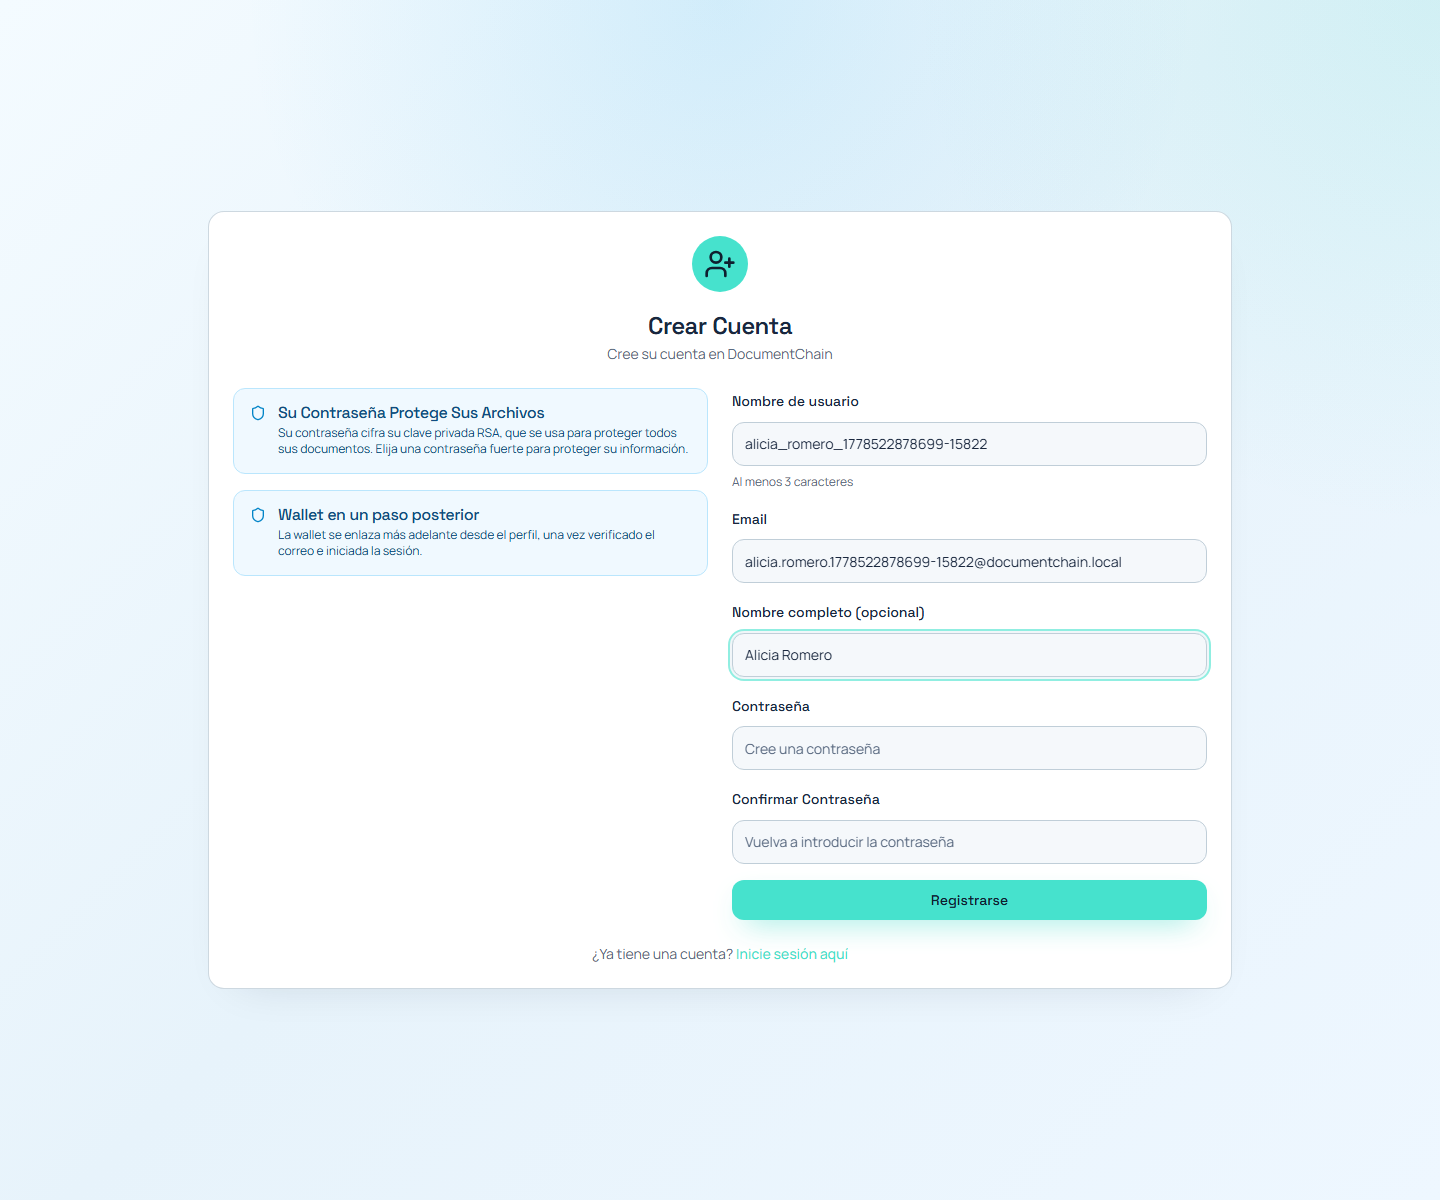
\includegraphics[width=0.8\textwidth]{capturas-ui/register-form.png}
    \caption{Formulario de registro}
    \label{fig:registro}
\end{figure}

\textbf{Resultado esperado}: la cuenta queda creada en estado activo y el usuario puede acceder al panel principal. Si el correo no se verifica, el sistema permitir\'{a} el login pero bloquear\'{a} ciertas acciones.

\textbf{Posibles errores y soluciones}:
\begin{itemize}
    \item \textit{``El nombre de usuario ya est\'{a} en uso''}: elija otro nombre \'{u}nico.
    \item \textit{``La contrase\~{n}a no cumple los requisitos''}: revise que incluya may\'{u}scula, min\'{u}scula, n\'{u}mero y s\'{i}mbolo.
    \item \textit{``No se pudo enviar el email de verificaci\'{o}n''}: verifique que el correo introducido sea v\'{a}lido y revise su carpeta de spam antes de reintentar.
\end{itemize}

\textbf{Nota}: los documentos privados se protegen criptogr\'{a}ficamente y solo pueden descargarse con las credenciales adecuadas. Los documentos p\'{u}blicos se publican sin cifrar porque est\'{a}n destinados a ser accesibles mediante enlace compartible.

\subsection{Inicio de sesi\'{o}n}

\textbf{Prop\'{o}sito}: acceder de forma segura al panel de gesti\'{o}n documental.

\begin{enumerate}
    \item Acceda a la p\'{a}gina \texttt{/login} desde el enlace \textbf{Iniciar sesi\'{o}n} en la pantalla de bienvenida.
    \item Introduzca su \textbf{correo electr\'{o}nico} o \textbf{nombre de usuario} y su \textbf{contrase\~{n}a}.
    \item Pulse \textbf{Acceder}.
\end{enumerate}

\begin{figure}[H]
    \centering
    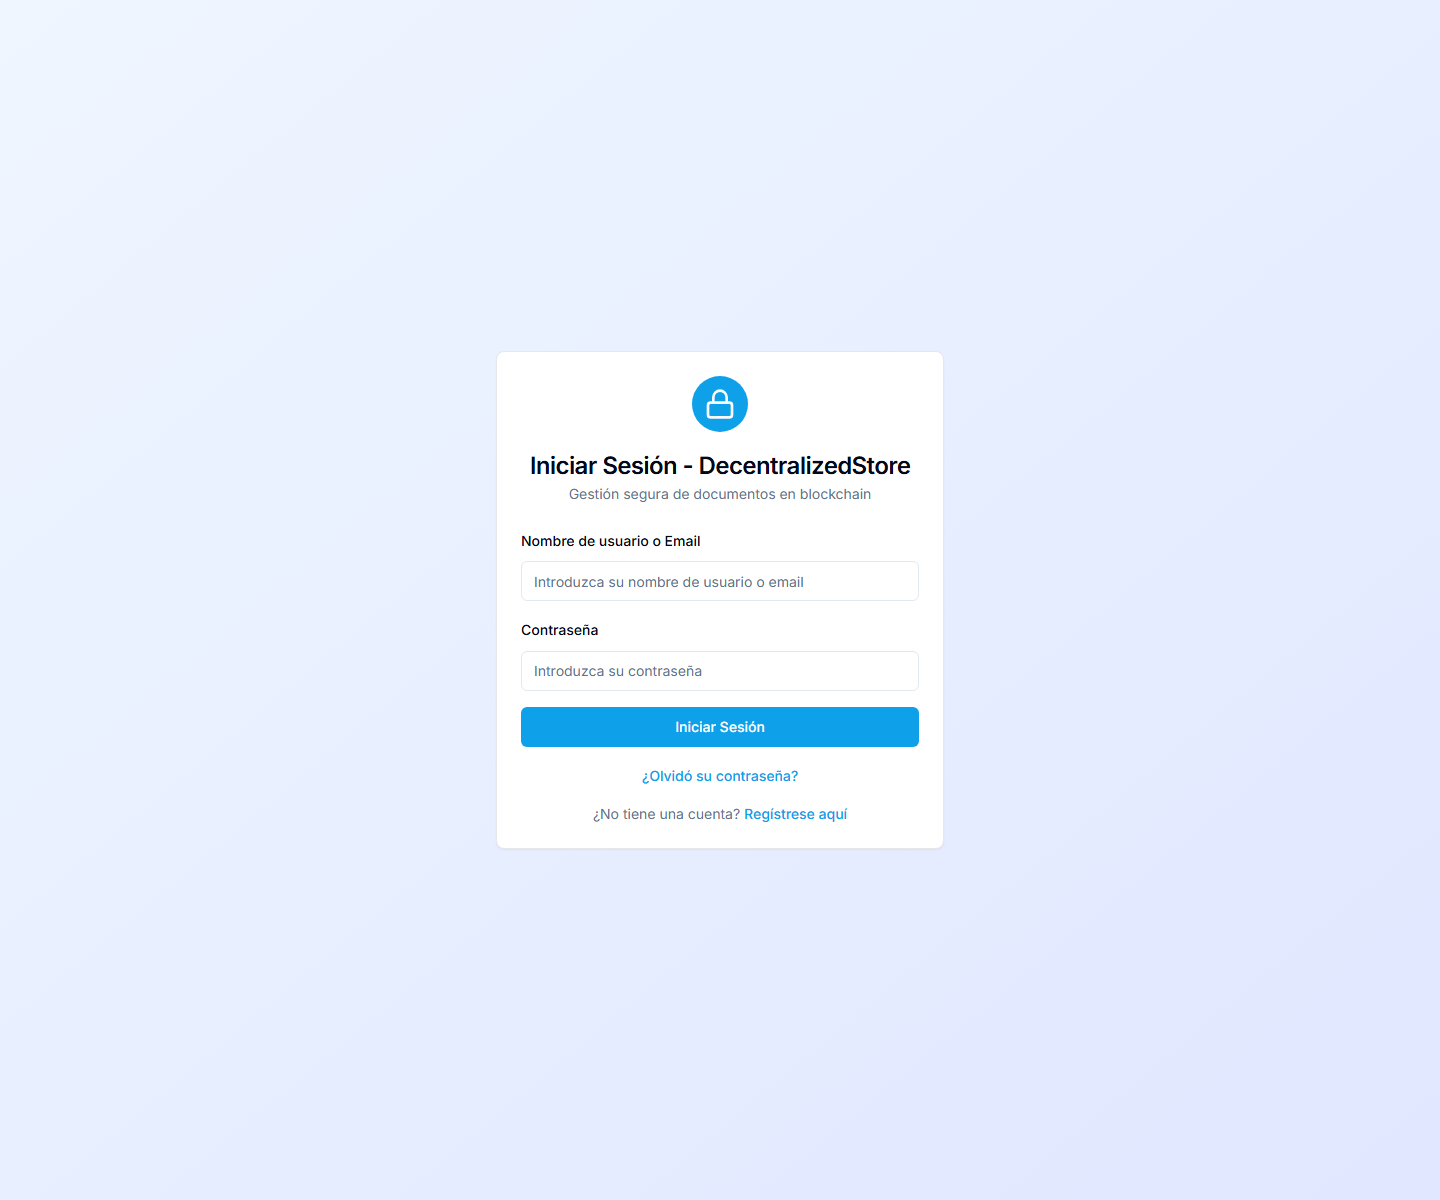
\includegraphics[width=0.8\textwidth]{capturas-ui/login-page.png}
    \caption{P\'{a}gina de inicio de sesi\'{o}n}
    \label{fig:login}
\end{figure}

\textbf{Resultado esperado}: el sistema redirige a \texttt{/app/documents}, la vista principal de documentos.

\textbf{Posibles errores y soluciones}:
\begin{itemize}
    \item \textit{``Credenciales inv\'{a}lidas''}: verifique may\'{u}sculas y min\'{u}sculas en la contrase\~{n}a. Si olvid\'{o} sus datos, utilice la recuperaci\'{o}n de contrase\~{n}a.
    \item \textit{``Cuenta no disponible''}: verifique que la cuenta sigue activa y contacte con el administrador del sistema si el problema persiste.
\end{itemize}

\subsection{Cerrar sesi\'{o}n}

\textbf{Prop\'{o}sito}: finalizar la sesi\'{o}n activa de forma segura.

\begin{enumerate}
    \item En la barra de navegaci\'{o}n superior, pulse sobre su avatar o nombre de usuario.
    \item Seleccione la opci\'{o}n \textbf{Cerrar sesi\'{o}n}.
    \item El sistema invalidar\'{a} sus tokens de acceso y le redirigir\'{a} a la p\'{a}gina de inicio.
    \item Si ten\'{i}a una wallet conectada, la conexi\'{o}n se cerrar\'{a} autom\'{a}ticamente.
\end{enumerate}

\subsection{Verificaci\'{o}n de correo electr\'{o}nico y reenv\'{i}o}

Tras completar el registro, o cuando se cambia la direcci\'{o}n de correo desde la configuraci\'{o}n de la cuenta, el sistema env\'{i}a un enlace de verificaci\'{o}n a la ruta \texttt{/verify-email}.

\begin{enumerate}
    \item Abra el mensaje recibido en su bandeja de entrada.
    \item Pulse el enlace de verificaci\'{o}n incluido en el cuerpo del mensaje.
    \item La pantalla mostrar\'{a} uno de los siguientes resultados:
    \begin{itemize}
        \item \textbf{Verificaci\'{o}n correcta}: la cuenta queda confirmada y ya puede iniciar sesi\'{o}n con normalidad.
        \item \textbf{Verificaci\'{o}n pendiente}: si la cuenta ya tiene sesi\'{o}n iniciada pero sigue bloqueada, la interfaz avisar\'{a} de que falta confirmar el correo y ofrecer\'{a} un bot\'{o}n de reenv\'{i}o.
        \item \textbf{Error de verificaci\'{o}n}: si el token no es v\'{a}lido, ha caducado o falta en la URL, se mostrar\'{a} un aviso y la opci\'{o}n de solicitar un nuevo mensaje.
    \end{itemize}
\end{enumerate}

\textbf{Soluci\'{o}n si no llega el correo}:
\begin{enumerate}
    \item Revise la carpeta de \textit{spam} o \textit{correo no deseado}.
    \item Espere al menos dos minutos antes de reenviar.
    \item Pulse \textbf{Reenviar email de verificaci\'{o}n} desde la pantalla de login o desde la notificaci\'{o}n de la interfaz.
    \item Si el problema persiste, verifique que su proveedor de correo no est\'{e} bloqueando los mensajes del remitente del sistema.
\end{enumerate}

\subsection{Recuperaci\'{o}n de contrase\~{n}a}

\textbf{Prop\'{o}sito}: restablecer el acceso cuando se ha olvidado la contrase\~{n}a.

\begin{enumerate}
    \item En la pantalla de inicio de sesi\'{o}n, haga clic en \textbf{Olvidaste tu contrase\~{n}a?}.
    \item Introduzca el \textbf{correo electr\'{o}nico} registrado en su cuenta.
    \item Recibir\'{a} un email con un enlace de recuperaci\'{o}n v\'{a}lido durante 1 hora.
    \item Haga clic en el enlace. Se abrir\'{a} una p\'{a}gina para crear una nueva contrase\~{n}a.
    \item Introduzca su \textbf{Recovery Key} (la clave que guard\'{o} al registrarse).
    \item Cree una nueva contrase\~{n}a que cumpla los requisitos de seguridad y conf\'{i}rmela.
    \item Pulse \textbf{Restablecer Contrase\~{n}a}.
\end{enumerate}

\textbf{Resultado esperado}: la contrase\~{n}a se actualiza y puede iniciar sesi\'{o}n con las nuevas credenciales.

\textbf{Advertencia cr\'{i}tica}: si no dispone de la Recovery Key, no ser\'{a} posible recuperar la cuenta ni descifrar sus documentos privados. En ese caso, deber\'{a} crear una nueva cuenta. Los documentos p\'{u}blicos permanecer\'{a}n accesibles si conserva sus enlaces.

\subsection{Seguridad de cuenta y eliminaci\'{o}n}

\textbf{Prop\'{o}sito}: mantener el acceso protegido y, cuando proceda, tramitar la baja definitiva de la cuenta.

\subsubsection{Eliminar cuenta permanentemente}

\textbf{Prop\'{o}sito}: borrar la cuenta y todos los datos asociados del sistema.

\begin{enumerate}
    \item Acceda a \textbf{Configuraci\'{o}n} $>$ \textbf{Cuenta}.
    \item Pulse \textbf{Eliminar cuenta}.
    \item Confirme la eliminaci\'{o}n con su contrase\~{n}a y, si es necesario, firme una transacci\'{o}n blockchain para registrar la baja de forma inmutable.
\end{enumerate}

\textbf{Advertencia}: la eliminaci\'{o}n es irreversible. Los registros en blockchain permanecer\'{a}n como evidencia hist\'{o}rica, pero los datos personales y los documentos cifrados se eliminar\'{a}n de la base de datos y de IPFS.

\begin{figure}[H]
    \centering
    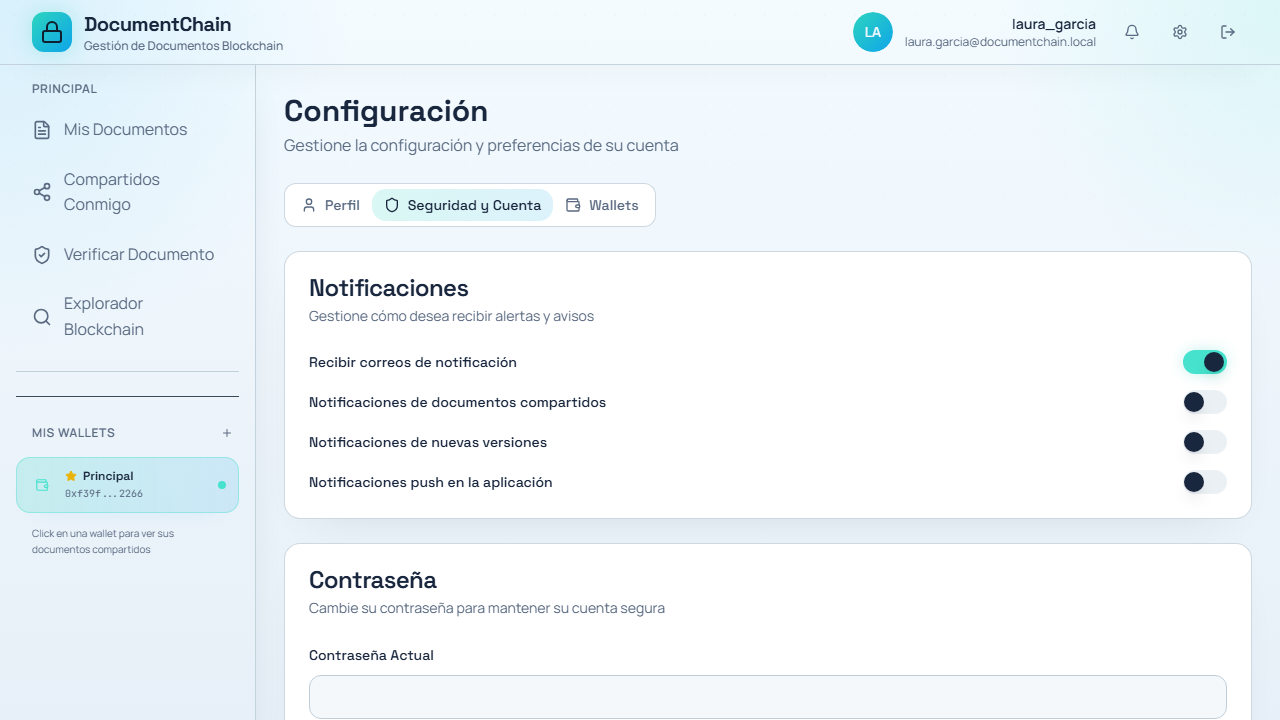
\includegraphics[width=0.8\textwidth]{capturas-ui/security-account-page.png}
    \caption{Pesta\~{n}a de seguridad y cuenta}
    \label{fig:security-account-page}
\end{figure}

\begin{figure}[H]
    \centering
    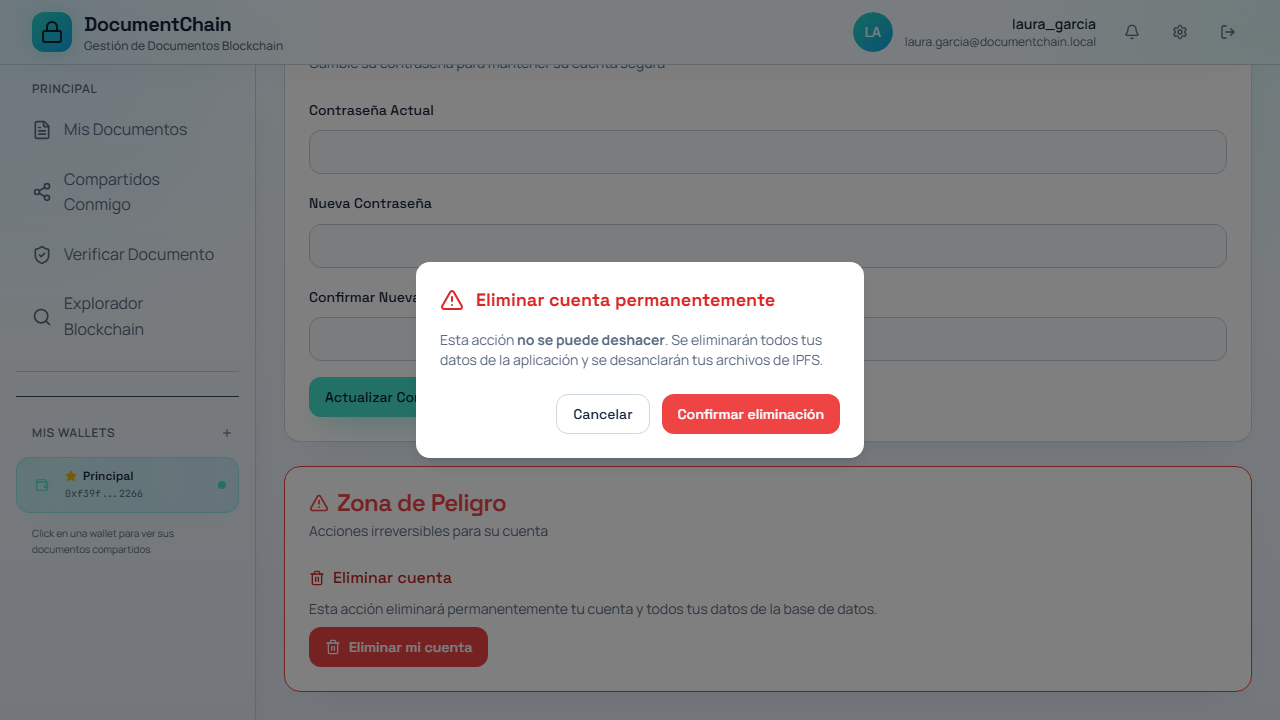
\includegraphics[width=0.72\textwidth]{capturas-ui/security-delete-confirmation.png}
    \caption{Confirmaci\'{o}n de eliminaci\'{o}n de cuenta}
    \label{fig:security-delete-confirmation}
\end{figure}

% ============================================================
\section{Gesti\'{o}n de documentos}
% ============================================================

Este apartado describe c\'{o}mo utilizar las funcionalidades principales relacionadas con los documentos: visualizaci\'{o}n, subida, b\'{u}squeda, descarga, edici\'{o}n, archivado, eliminaci\'{o}n y transferencia de propiedad.

\subsection{Vista principal de documentos}

Tras iniciar sesi\'{o}n, el sistema redirige a \texttt{/app/documents}, que act\'{u}a como punto de entrada principal.

\subsubsection{Elementos principales}

\begin{enumerate}
    \item \textbf{Cabecera superior}:
    \begin{itemize}
        \item Identidad visual de DocumentChain.
        \item Informaci\'{o}n resumida de la sesi\'{o}n del usuario.
        \item Accesos directos a \textbf{Notificaciones}, \textbf{Configuraci\'{o}n} y \textbf{Cerrar sesi\'{o}n}.
    \end{itemize}
    \item \textbf{Barra lateral izquierda}:
    \begin{itemize}
        \item \textbf{Mis Documentos}: colecci\'{o}n propia del usuario.
        \item \textbf{Compartidos Conmigo}: documentos accesibles con la wallet activa.
        \item \textbf{Verificar Documento}: herramienta de comprobaci\'{o}n manual.
        \item \textbf{Explorador Blockchain}: visor t\'{e}cnico de eventos y transacciones.
        \item \'{A}rbol de \textbf{carpetas} cuando se est\'{a} en la vista de documentos.
        \item Widget de \textbf{almacenamiento} utilizado.
        \item Selector de \textbf{wallets guardadas}.
    \end{itemize}
    \item \textbf{Área principal}:
    \begin{itemize}
        \item Botones \textbf{Nueva Carpeta} y \textbf{Subir Documento}.
        \item Pesta\~{n}as \textbf{Activos} y \textbf{Archivados}.
        \item B\'{u}squeda por nombre y filtro por tipo de archivo.
        \item Listado paginado de documentos con acceso directo al detalle.
    \end{itemize}
\end{enumerate}

\begin{figure}[H]
    \centering
    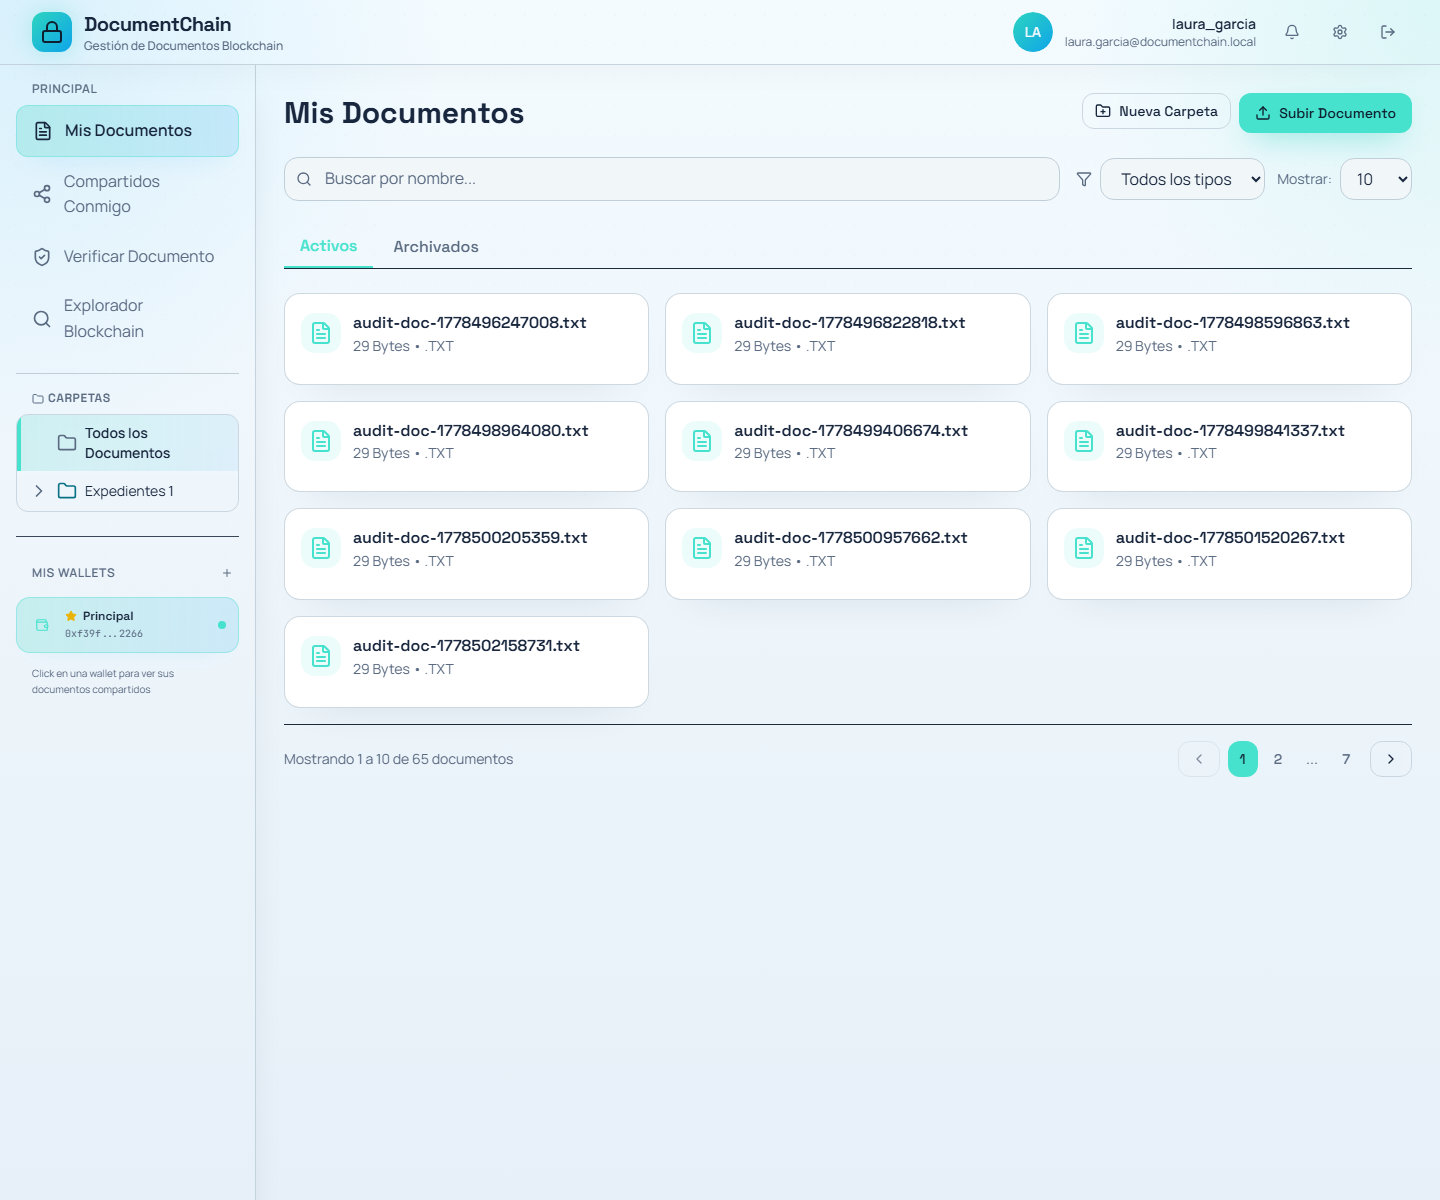
\includegraphics[width=0.9\textwidth]{capturas-ui/documents-page.png}
    \caption{Vista principal de documentos}
    \label{fig:documents-page-main}
\end{figure}

\subsection{Subir un documento}

\textbf{Prop\'{o}sito}: registrar un archivo en el sistema, almacenarlo de forma segura en IPFS y anclar su hash en blockchain para garantizar su inmutabilidad.

\begin{enumerate}
    \item Haga clic en el bot\'{o}n \textbf{+ Subir Documento} situado en el \'{a}rea principal del panel.
    \item Se abrir\'{a} un modal con un formulario. Puede aportar el archivo de dos maneras:
    \begin{itemize}
        \item \textbf{Arrastrar y soltar} (drag \& drop): arrastre el archivo hasta la zona delimitada en el modal.
        \item \textbf{Selecci\'{o}n manual}: haga clic en \textbf{Seleccionar archivo} y b\'{u}squelo en su ordenador.
    \end{itemize}
    \item Complete la informaci\'{o}n del formulario:
    \begin{itemize}
        \item \textbf{Nombre del documento}: identificativo obligatorio (m\'{a}ximo 100 caracteres).
        \item \textbf{Descripci\'{o}n} (opcional): contexto o resumen del contenido.
        \item \textbf{Carpeta} (opcional): seleccione una carpeta existente o cree una nueva para organizar el archivo.
        \item \textbf{Etiquetas} (opcional): a\~{n}ada t\'{e}rminos separados por comas para facilitar la b\'{u}squeda posterior.
        \item \textbf{Visibilidad}: elija entre \textbf{Privado} (cifrado, solo accesible para usted y quienes comparta) o \textbf{P\'{u}blico} (accesible mediante enlace y QR).
    \end{itemize}
    \item Si activa la opci\'{o}n \textbf{Publicar documento con enlace y QR}, la interfaz mostrar\'{a} una advertencia: ese archivo se almacenar\'{a} sin cifrar y cualquier persona con el enlace podr\'{a} visualizarlo o descargarlo.
    \item Pulse \textbf{Subir y Firmar}. El sistema preparar\'{a} el documento seg\'{u}n la visibilidad elegida y solicitar\'{a} una wallet para firmar la operaci\'{o}n blockchain.
    \item Confirme la transacci\'{o}n en la wallet conectada y espere a que el registro cambie al estado \textbf{Sincronizado}.
    \item Cuando finalice el proceso, el documento aparecer\'{a} en la lista principal.
\end{enumerate}

\begin{figure}[H]
    \centering
    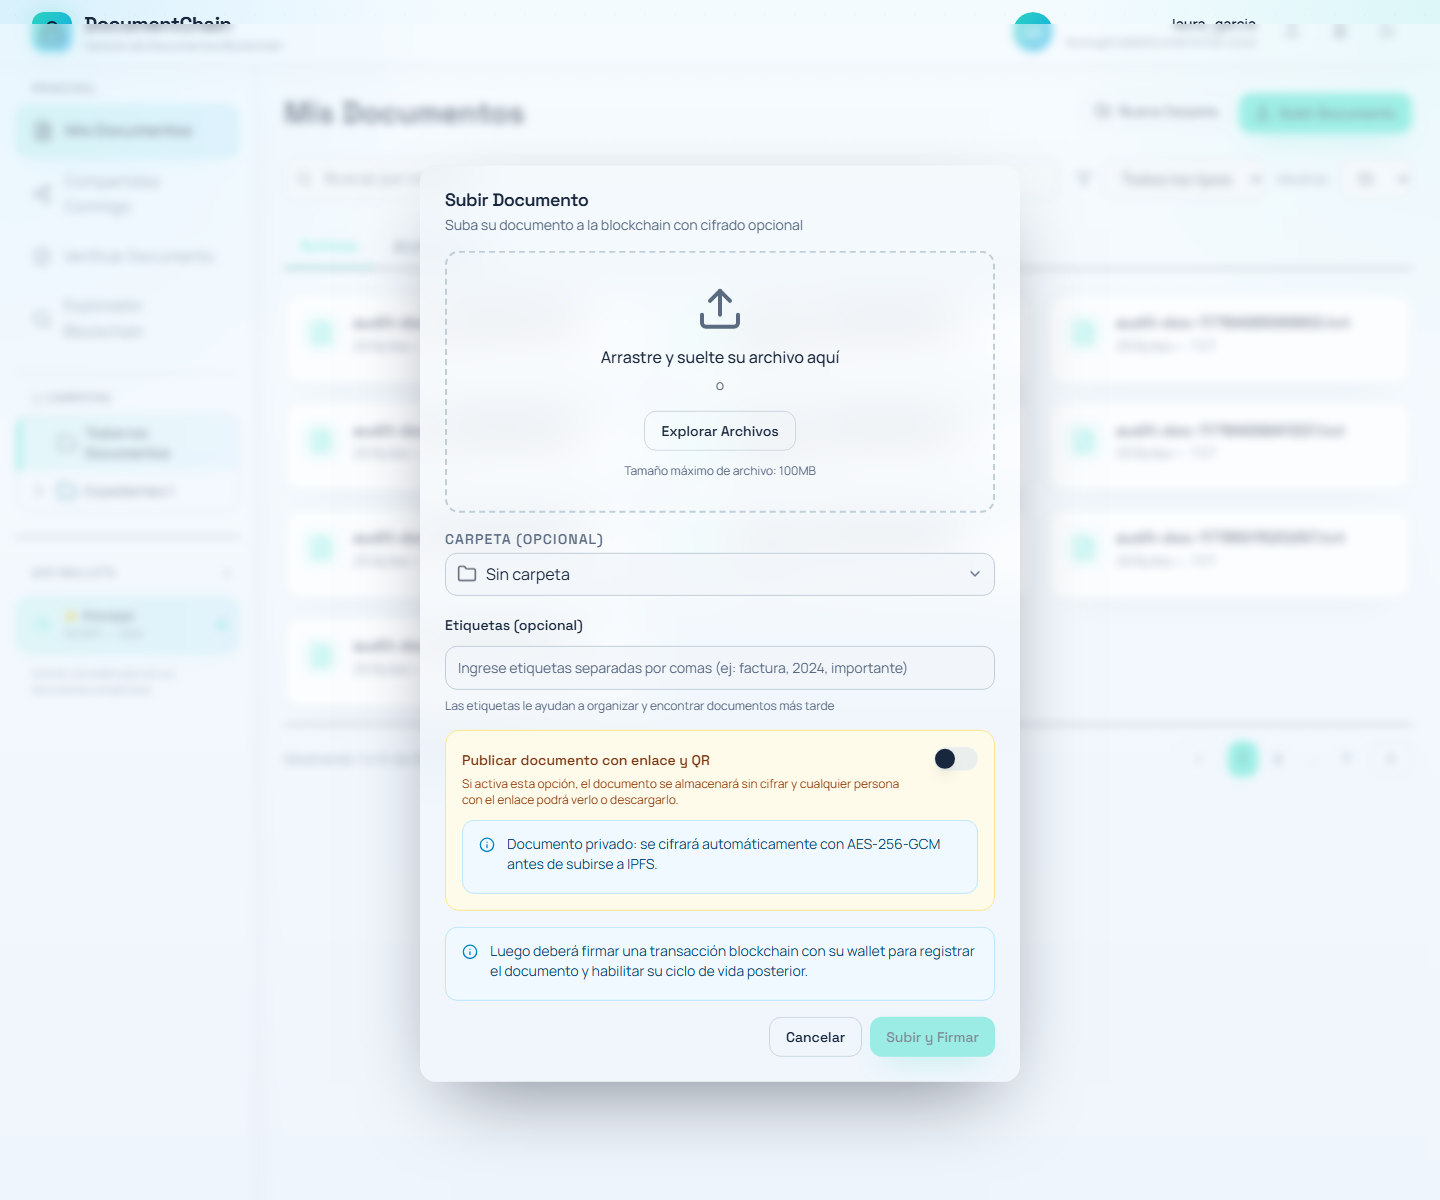
\includegraphics[width=0.8\textwidth]{capturas-ui/upload-modal.png}
    \caption{Modal de subida de documento}
    \label{fig:upload}
\end{figure}

\textbf{Resultado esperado}: el documento se almacena en IPFS, su metadato se registra en blockchain y se genera una entrada en la base de datos local con el estado correspondiente.

\textbf{Posibles errores y soluciones}:
\begin{itemize}
    \item \textit{``El archivo excede el l\'{i}mite de 100 MB''}: reduzca el tama\~{n}o del archivo o div\'{i}dalo en vol\'{u}menes menores.
    \item \textit{``Firma rechazada en la wallet''}: si cancela la transacci\'{o}n, el documento quedar\'{a} en estado \textbf{Preparando}. Puede reintentar la firma desde el detalle del documento.
    \item \textit{``IPFS no disponible''}: el nodo de almacenamiento puede estar saturado. Espere unos segundos y reintente la subida.
\end{itemize}

\textbf{Consejo}: si la firma o la confirmaci\'{o}n fallan, el propio asistente de subida mostrar\'{a} el estado alcanzado para que pueda repetir la operaci\'{o}n.

\subsection{Buscar documentos}

\textbf{Prop\'{o}sito}: localizar r\'{a}pidamente uno o varios documentos mediante filtros combinados.

La barra de b\'{u}squeda del panel principal permite filtrar por:

\begin{itemize}
    \item \textbf{Nombre}: coincidencia parcial con el t\'{i}tulo del documento.
    \item \textbf{Tipo de archivo}: extensi\'{o}n (PDF, DOCX, PNG, etc.).
    \item \textbf{Fecha de subida}: rango de fechas (desde/hasta).
    \item \textbf{Etiquetas}: documentos que contengan alguna de las etiquetas indicadas.
    \item \textbf{Estado blockchain}: \textbf{Preparando}, \textbf{Confirmando} o \textbf{Sincronizado}.
    \item \textbf{Carpeta}: contenido dentro de una carpeta espec\'{i}fica.
\end{itemize}

Los resultados se actualizan en tiempo real a medida que se introducen criterios. Puede combinar varios filtros para refinar la b\'{u}squeda.

\textbf{Resultado esperado}: listado paginado de documentos que cumplen los criterios, ordenados por fecha de modificaci\'{o}n descendente.

\subsection{Descargar un documento}

\textbf{Prop\'{o}sito}: recuperar el archivo original en su dispositivo local.

\begin{enumerate}
    \item Localice el documento en la lista principal o mediante la b\'{u}squeda.
    \item Haga clic en el bot\'{o}n \textbf{Descargar} (icono de flecha hacia abajo) o abra el detalle del documento y seleccione \textbf{Descargar versi\'{o}n operativa}.
    \item Si el documento es privado, el navegador utilizar\'{a} su clave privada local para descifrar el contenido recibido desde IPFS de forma transparente.
    \item Elija la ubicaci\'{o}n de guardado en su dispositivo.
\end{enumerate}

\textbf{Resultado esperado}: el archivo se descarga en su formato original.

\textbf{Posibles errores}:
\begin{itemize}
    \item \textit{``No tiene permisos de lectura''}: verifique que es el propietario o que el documento ha sido compartido con usted.
    \item \textit{``Error de descifrado''}: si borr\'{o} los datos de navegaci\'{o}n (localStorage) o utiliza otro dispositivo, es posible que falte la clave privada local necesaria para descifrar. Use la Recovery Key para restaurarla.
\end{itemize}

\begin{figure}[H]
    \centering
    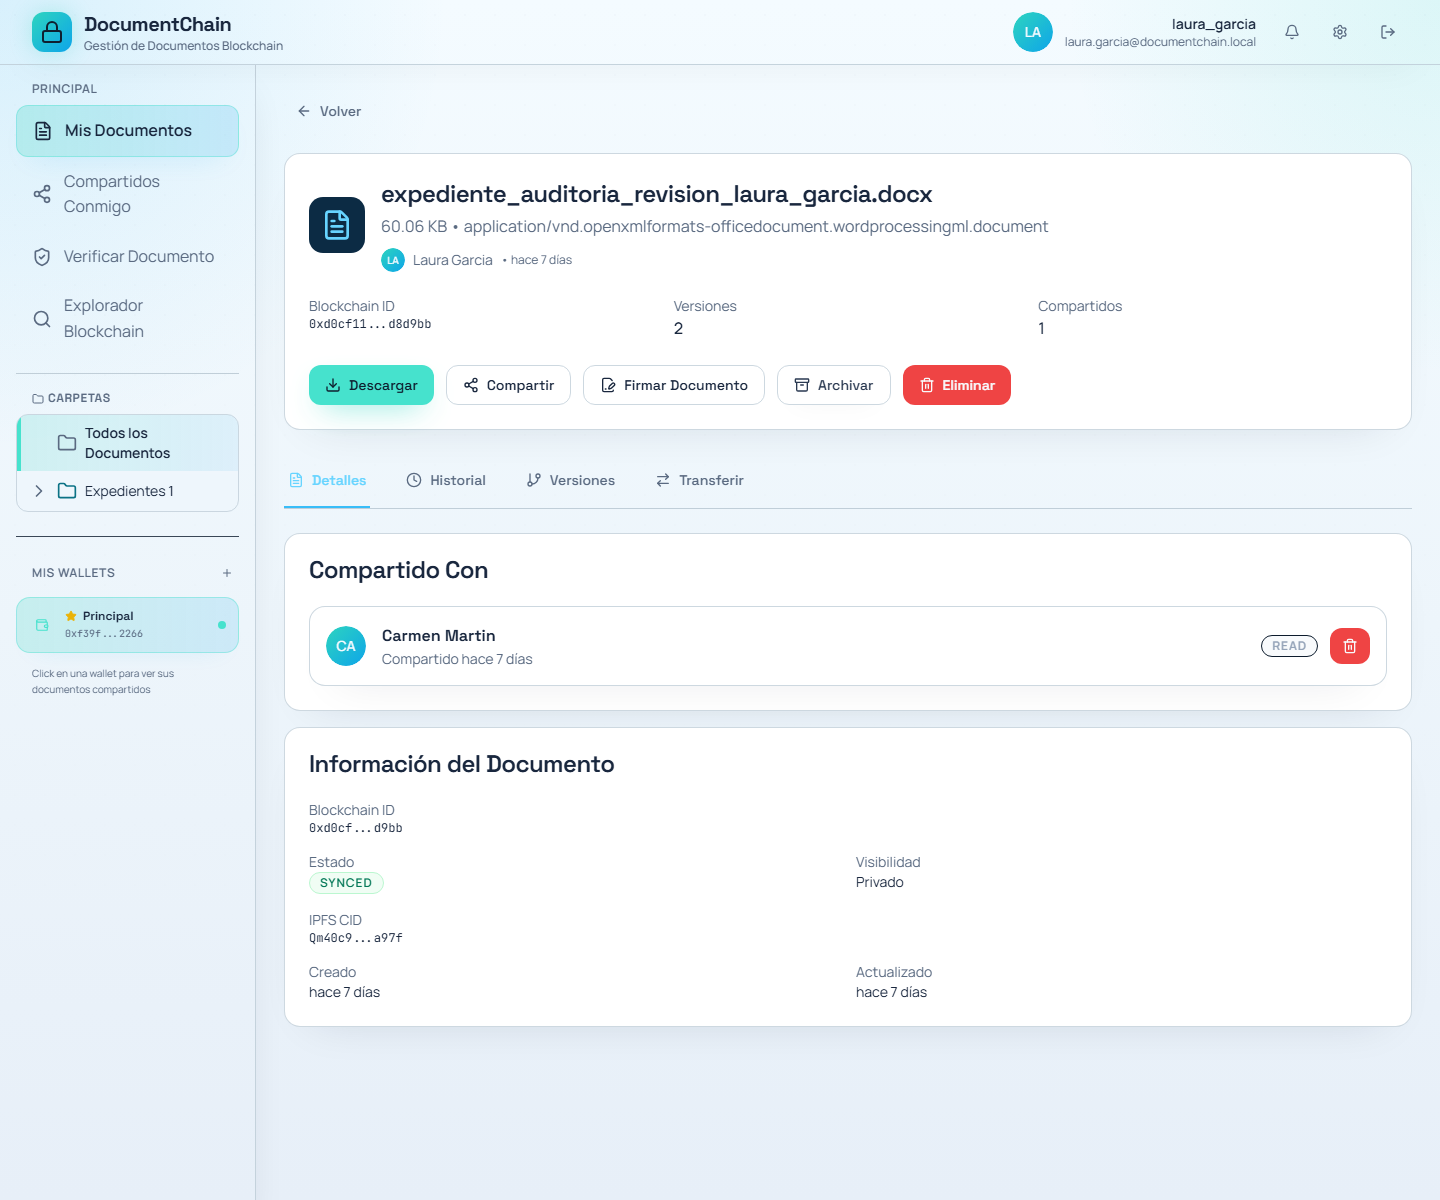
\includegraphics[width=0.88\textwidth]{capturas-ui/document-detail.png}
    \caption{Detalle de documento con acciones operativas}
    \label{fig:document-detail-main}
\end{figure}

\begin{figure}[H]
    \centering
    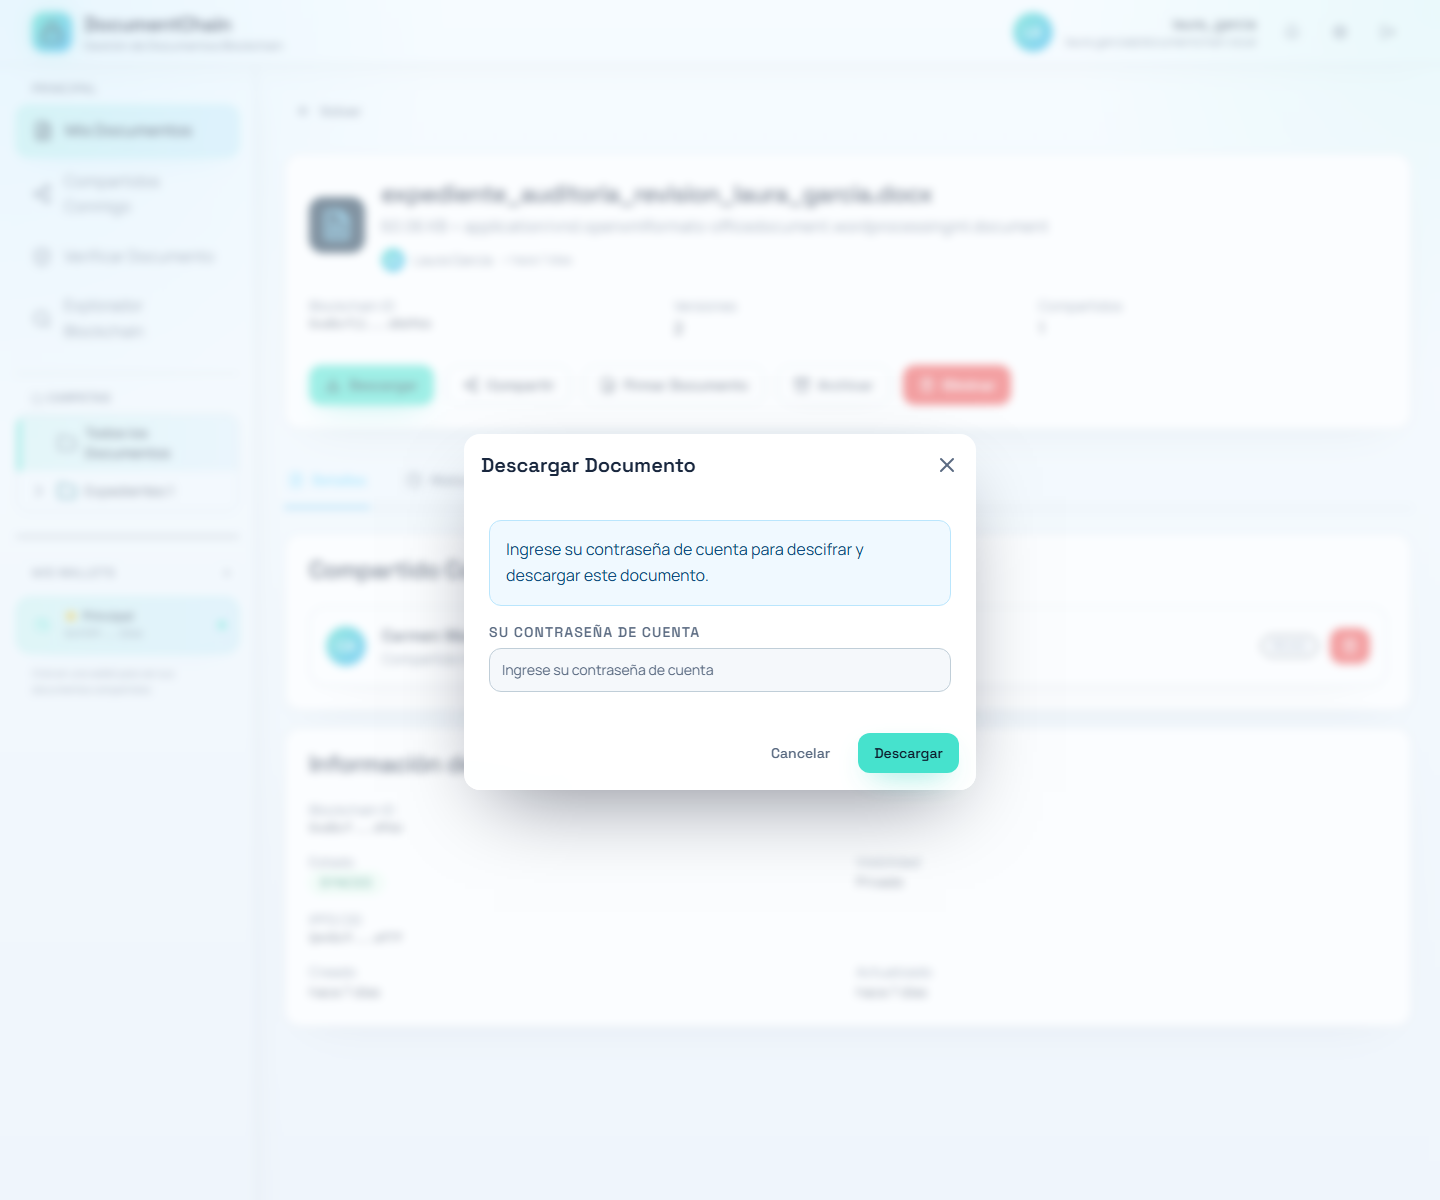
\includegraphics[width=0.72\textwidth]{capturas-ui/download-modal.png}
    \caption{Modal de descarga de documento}
    \label{fig:download-modal-main}
\end{figure}

\subsection{Editar metadatos}

\textbf{Prop\'{o}sito}: modificar la informaci\'{o}n descriptiva de un documento sin alterar su contenido ni su registro en blockchain.

\begin{enumerate}
    \item Abra el detalle del documento haciendo clic en su nombre.
    \item Pulse el icono de edici\'{o}n (l\'{a}piz) junto a los campos \textbf{Nombre}, \textbf{Descripci\'{o}n} o \textbf{Etiquetas}.
    \item Realice los cambios deseados.
    \item Pulse \textbf{Guardar cambios}.
\end{enumerate}

\textbf{Nota}: los cambios en metadatos se almacenan en la base de datos local. Si desea registrar la modificaci\'{o}n de forma inmutable en blockchain, deber\'{a} crear una nueva versi\'{o}n del documento.

\subsection{Transferir propiedad}

Para transferir la propiedad de un documento a otro usuario:

\begin{enumerate}[nosep,leftmargin=*]
    \item Acceda al detalle del documento y seleccione la pestana \textbf{Transferir}.
    \item Introduzca la direccion de correo electronico del nuevo propietario.
    \item El sistema verificara que el destinatario esta registrado en DocumentChain.
    \item Confirme la transferencia. La operacion requiere firma mediante su wallet.
    \item Una vez confirmada, el nuevo propietario recibira una notificacion y el documento aparecera en su lista principal.
\end{enumerate}

\begin{figure}[H]
    \centering
    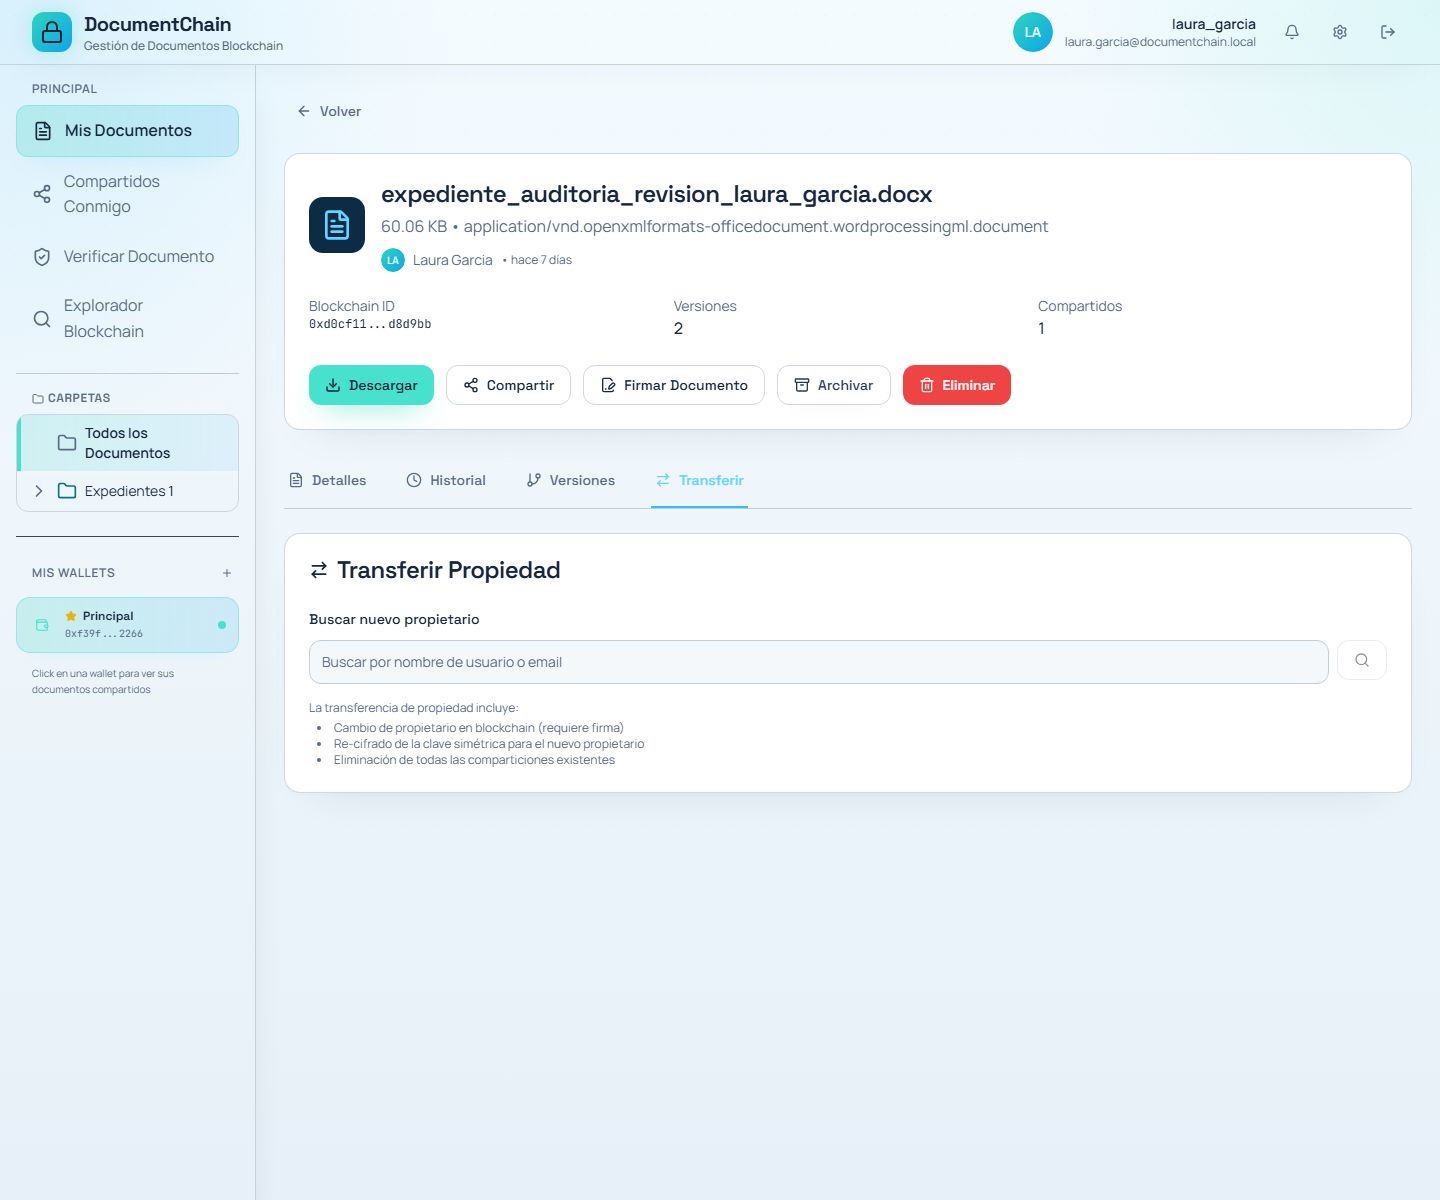
\includegraphics[width=0.72\textwidth]{capturas-ui/transfer-tab.png}
    \caption{Pestana de transferencia de propiedad}
    \label{fig:transfer-tab}
\end{figure}

\textbf{Resultado esperado}: el documento desaparece de su lista de documentos propios y pasa a la del nuevo titular.

\subsection{Archivar y eliminar}

\textbf{Prop\'{o}sito}: organizar el espacio de trabajo eliminando de la vista aquellos documentos que ya no son prioritarios, ya sea de forma reversible (archivar) o definitiva (eliminaci\'{o}n l\'{o}gica).

\begin{itemize}
    \item \textbf{Archivar}: el documento desaparece de la pesta\~{n}a \textbf{Activos} y pasa a \textbf{Archivados}. Puede desarchivarlo en cualquier momento desde la misma pesta\~{n}a. El archivo permanece cifrado y accesible.
    \item \textbf{Eliminar}: el documento se marca como eliminado l\'{o}gicamente. El registro permanece en blockchain como evidencia hist\'{o}rica, pero deja de ser visible en la interfaz y no puede descargarse. Esta acci\'{o}n suele requerir confirmaci\'{o}n adicional y, en algunos casos, firma blockchain.
\end{itemize}

\begin{table}[H]
\centering
\caption{Diferencias entre archivar y eliminar}
\label{tab:archivar-eliminar}
\begin{tabular}{@{}lp{5cm}p{5cm}@{}}
\toprule
\textbf{Caracter\'{i}stica} & \textbf{Archivar} & \textbf{Eliminar} \\
\midrule
Visibilidad en lista & Pasa a ``Archivados'' & Desaparece de la interfaz \\
Acceso al contenido & S\'{i}, mediante desarchivado & No, salvo registro blockchain \\
Reversibilidad & Reversible & Irreversible desde la interfaz \\
Registro blockchain & Sin cambios & Mantiene el hash hist\'{o}rico \\
\bottomrule
\end{tabular}
\end{table}

\subsection{Gesti\'{o}n de carpetas}

\textbf{Prop\'{o}sito}: organizar los documentos en carpetas jer\'{a}rquicas.

\begin{enumerate}
    \item En la vista principal de documentos, localice el panel lateral de carpetas.
    \item Para \textbf{crear una carpeta}, pulse el bot\'{o}n \textbf{+ Nueva carpeta}, introduzca un nombre y confirme.
    \item Para \textbf{mover documentos} a una carpeta, seleccione los documentos mediante las casillas de verificaci\'{o}n y arr\'{a}strelos a la carpeta destino, o utilice la opci\'{o}n \textbf{Mover a...} del men\'{u} de acciones.
    \item Para \textbf{renombrar o eliminar} una carpeta, pulse el icono de configuraci\'{o}n junto al nombre de la carpeta y seleccione la acci\'{o}n deseada.
    \item Las carpetas pueden anidarse para crear una estructura jer\'{a}rquica.
\end{enumerate}

% ============================================================
\section{Versiones}
% ============================================================

En este apartado se describe como gestionar el historial de versiones de los documentos en DocumentChain.

El sistema mantiene un historial inmutable de versiones para cada documento. Cada vez que se crea una nueva versi\'{o}n, el sistema genera un nuevo identificador de contenido (CID) en IPFS y un nuevo registro en blockchain. Las versiones anteriores no se sobrescriben; permanecen accesibles en el historial.

\subsection{Historial de versiones}

\textbf{Prop\'{o}sito}: consultar la evoluci\'{o}n temporal de un documento.

\begin{enumerate}
    \item Abra el detalle del documento.
    \item Seleccione la pesta\~{n}a \textbf{Versiones}.
    \item Se mostrar\'{a} una tabla con todas las versiones registradas, indicando:
    \begin{itemize}
        \item N\'{u}mero de versi\'{o}n.
        \item Fecha y hora de creaci\'{o}n.
        \item Hash IPFS (CID).
        \item Transacci\'{o}n blockchain asociada.
        \item Indicador de \textbf{versi\'{o}n operativa} (la que se utiliza actualmente).
    \end{itemize}
\end{enumerate}

\begin{figure}[H]
    \centering
    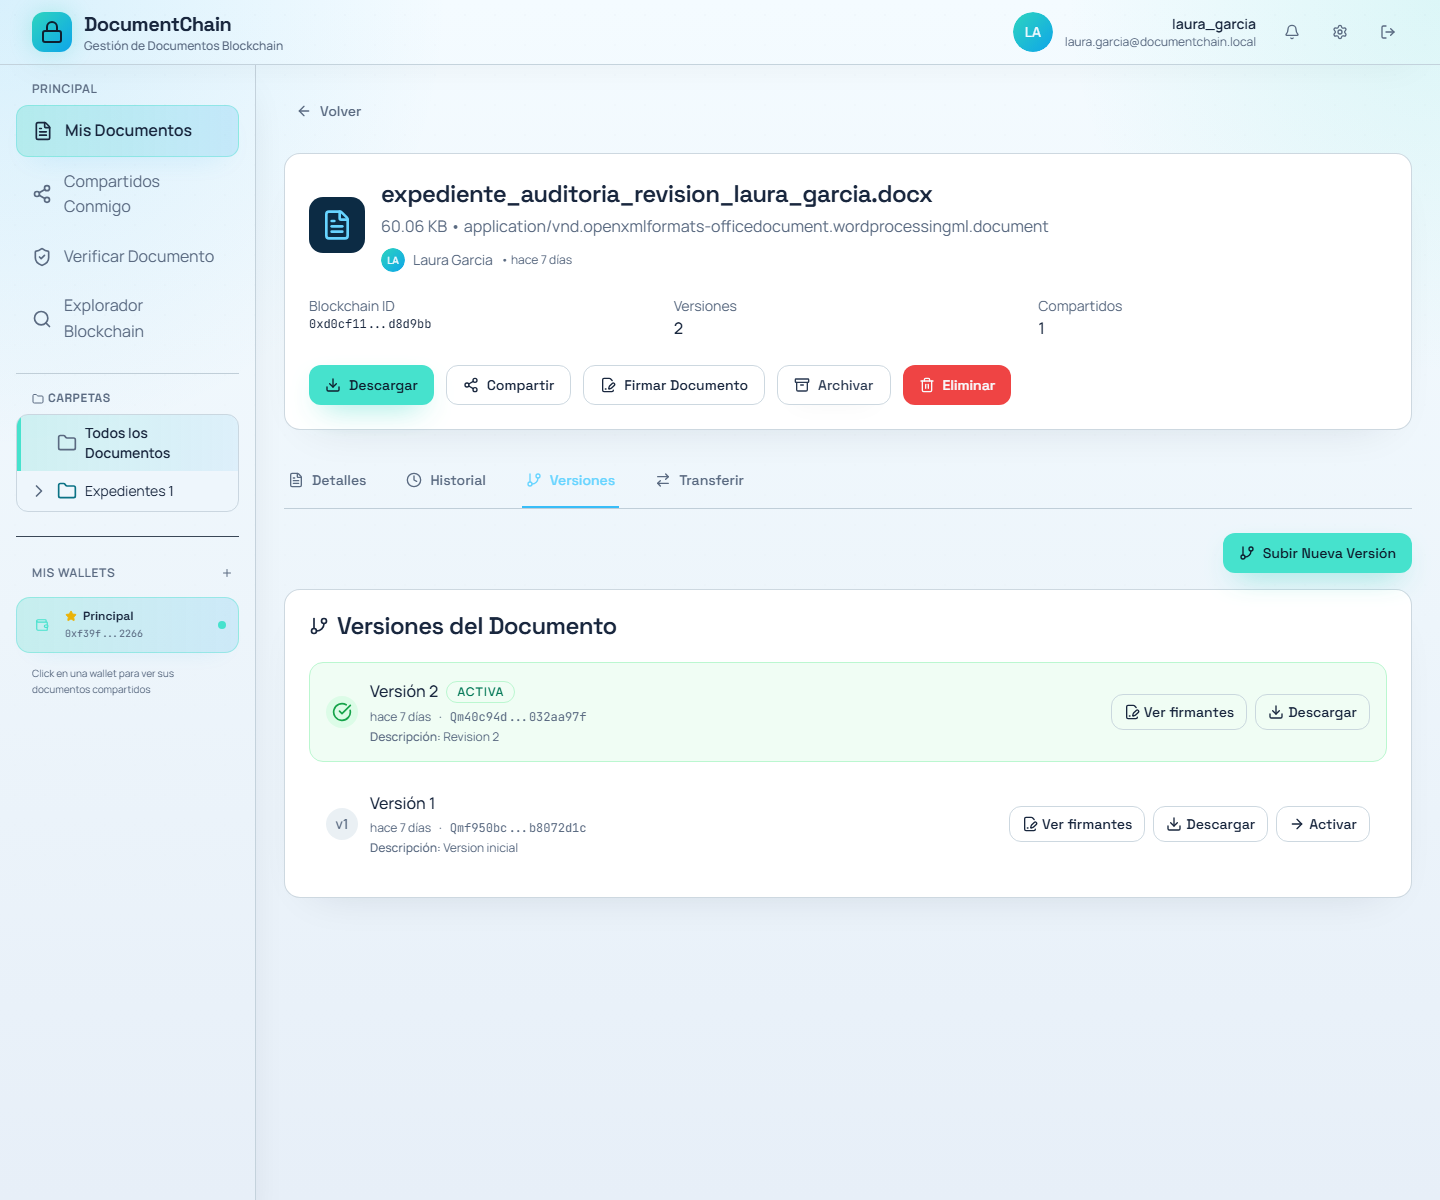
\includegraphics[width=0.8\textwidth]{capturas-ui/versions-tab.png}
    \caption{Pesta\~{n}a de versiones de un documento}
    \label{fig:versions}
\end{figure}

\subsection{Crear una nueva versi\'{o}n}

\textbf{Prop\'{o}sito}: actualizar el contenido de un documento conservando el historial completo.

\begin{enumerate}
    \item Abra el detalle del documento y vaya a \textbf{Versiones}.
    \item Pulse \textbf{Nueva Versi\'{o}n}.
    \item Seleccione el archivo actualizado desde su dispositivo.
    \item A\~{n}ada una nota de cambio (opcional) para describir las modificaciones realizadas.
    \item Confirme la subida y firme la transacci\'{o}n blockchain cuando se solicite.
\end{enumerate}

\textbf{Resultado esperado}: la nueva versi\'{o}n se a\~{n}ade al historial y se convierte autom\'{a}ticamente en la versi\'{o}n operativa.

\subsection{Establecer versi\'{o}n operativa}

\textbf{Prop\'{o}sito}: cambiar qu\'{e} versi\'{o}n del documento se considera la vigente sin crear una nueva entrada.

\begin{enumerate}
    \item En la pesta\~{n}a \textbf{Versiones}, localice la versi\'{o}n que desea activar.
    \item Pulse el bot\'{o}n \textbf{Establecer como operativa}.
    \item Confirme la acci\'{o}n.
\end{enumerate}

\textbf{Resultado esperado}: la versi\'{o}n seleccionada pasa a ser la que se muestra por defecto y la que se descarga al pulsar \textbf{Descargar}.

\subsection{Restaurar versi\'{o}n anterior}

\textbf{Prop\'{o}sito}: recuperar el contenido de una versi\'{o}n anterior como nueva versi\'{o}n operativa, preservando el historial.

\begin{enumerate}
    \item En la pesta\~{n}a \textbf{Versiones}, seleccione la versi\'{o}n antigua que desea recuperar.
    \item Pulse \textbf{Restaurar}.
    \item El sistema crear\'{a} autom\'{a}ticamente una nueva versi\'{o}n que reutiliza el contenido de la anterior, de modo que no se pierde ninguna entrada del historial.
    \item Firme la transacci\'{o}n blockchain si se solicita.
\end{enumerate}

\textbf{Resultado esperado}: el contenido antiguo vuelve a ser la versi\'{o}n operativa actual, pero la versi\'{o}n desde la que se restaur\'{o} sigue visible en el historial.

\subsection{Descargar versi\'{o}n espec\'{i}fica}

\textbf{Prop\'{o}sito}: obtener el archivo correspondiente a una versi\'{o}n concreta del historial.

\begin{enumerate}
    \item En la pesta\~{n}a \textbf{Versiones}, localice la fila deseada.
    \item Pulse el icono de descarga al final de la fila.
    \item El navegador descargar\'{a} el archivo asociado a esa versi\'{o}n.
\end{enumerate}

% ============================================================
\section{Firmas digitales}

En este apartado se explica como utilizar las firmas digitales con wallet Ethereum para demostrar la aprobacion de documentos.

Las firmas digitales en DocumentChain permiten demostrar la aprobaci\'{o}n de un documento mediante la firma criptogr\'{a}fica de un mensaje vinculado al hash del contenido, utilizando una wallet Ethereum.

\subsection{Firmar un documento}

\textbf{Prop\'{o}sito}: aportar una prueba inmutable de aprobaci\'{o}n o revisi\'{o}n del documento.

\begin{enumerate}
    \item Conecte su wallet (MetaMask, WalletConnect, etc.) y aseg\'{u}rese de que est\'{a} desbloqueada.
    \item Abra el detalle del documento y seleccione \textbf{Firmar}.
    \item Seleccione la wallet con la que desea firmar (si tiene varias guardadas).
    \item Revise el mensaje que se va a firmar. Contiene un resumen (hash) del documento y la marca temporal.
    \item Confirme la transacci\'{o}n en su wallet.
    \item Espere la confirmaci\'{o}n blockchain. La firma aparecer\'{a} en la pesta\~{n}a \textbf{Firmas} del documento.
\end{enumerate}

\begin{figure}[H]
    \centering
    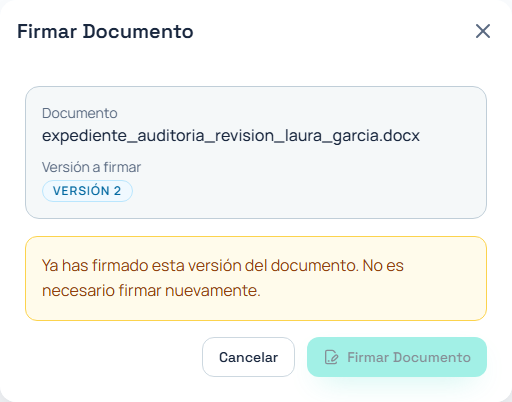
\includegraphics[width=0.8\textwidth]{capturas-ui/sign-modal.png}
    \caption{Modal de firma digital}
    \label{fig:sign}
\end{figure}

\textbf{Resultado esperado}: la firma queda registrada en el contrato inteligente y se visualiza en el detalle con la direcci\'{o}n del firmante, la fecha y el identificador de la transacci\'{o}n.

\textbf{Posibles errores y soluciones}:
\begin{itemize}
    \item \textit{``Wallet no conectada''}: pulse \textbf{Conectar wallet} en la cabecera y seleccione una wallet compatible.
    \item \textit{``Transacci\'{o}n rechazada''}: verifique que tiene saldo suficiente de ETH (gas) y que la red seleccionada es la correcta.
    \item \textit{``No se pudo sincronizar la firma''}: el nodo blockchain puede estar desfasado. Espere unos segundos y recargue la p\'{a}gina.
\end{itemize}

\subsection{Ver firmas asociadas}

\textbf{Prop\'{o}sito}: conocer qui\'{e}nes han firmado el documento y en qu\'{e} momento.

\begin{enumerate}
    \item Abra el detalle del documento.
    \item Vaya a la pesta\~{n}a \textbf{Firmas} o \textbf{Firmantes}.
    \item Se mostrar\'{a} una lista con:
    \begin{itemize}
        \item Direcci\'{o}n Ethereum del firmante.
        \item Fecha y hora UTC de la firma.
        \item Enlace al explorador blockchain para ver la transacci\'{o}n.
    \end{itemize}
\end{enumerate}

\begin{figure}[H]
    \centering
    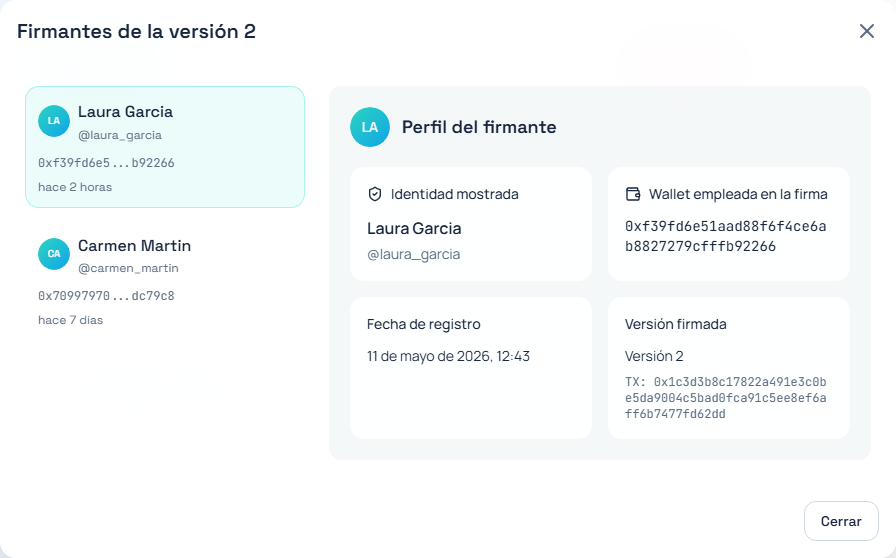
\includegraphics[width=0.8\textwidth]{capturas-ui/signers-modal.png}
    \caption{Modal de firmantes}
    \label{fig:signers}
\end{figure}

\subsection{Verificar firma del usuario}

\textbf{Prop\'{o}sito}: comprobar de forma independiente que una firma existe realmente en la blockchain.

\begin{enumerate}
    \item En la lista de firmas, pulse el enlace \textbf{Ver en blockchain} o copie el hash de la transacci\'{o}n.
    \item Se abrir\'{a} el explorador de bloques integrado (o una herramienta externa si la red es p\'{u}blica).
    \item Verifique que los datos del evento (direcci\'{o}n del firmante, hash del documento y timestamp) coinciden con lo mostrado en DocumentChain.
\end{enumerate}

\textbf{Resultado esperado}: confirmaci\'{o}n de que la firma es v\'{a}lida, no ha sido alterada y est\'{a} inmutablemente registrada.

% ============================================================
\section{Compartici\'{o}n}

En este apartado se describe como compartir documentos con otros usuarios del sistema mediante permisos basados en roles.

DocumentChain permite compartir documentos con otros usuarios del sistema mediante permisos basados en roles, registrados tanto en la base de datos como en el contrato inteligente de control de acceso.

\subsection{Compartir un documento}

\textbf{Prop\'{o}sito}: conceder acceso a otro usuario para que pueda leer o colaborar en un documento.

\begin{enumerate}
    \item Abra el detalle del documento que desea compartir.
    \item Pulse el bot\'{o}n \textbf{Compartir}.
    \item En el modal, introduzca la direcci\'{o}n de correo electr\'{o}nico, el nombre de usuario o la direcci\'{o}n de wallet del destinatario.
    \item Seleccione el \textbf{rol}:
    \begin{itemize}
        \item \textbf{Lector}: puede visualizar y descargar el documento.
        \item \textbf{Editor}: adem\'{a}s de leer, puede modificar metadatos y subir nuevas versiones.
    \end{itemize}
    \item Confirme la compartici\'{o}n.
    \item Si el sistema lo requiere, firme la transacci\'{o}n blockchain para registrar el permiso de forma inmutable.
\end{enumerate}

\begin{figure}[H]
    \centering
    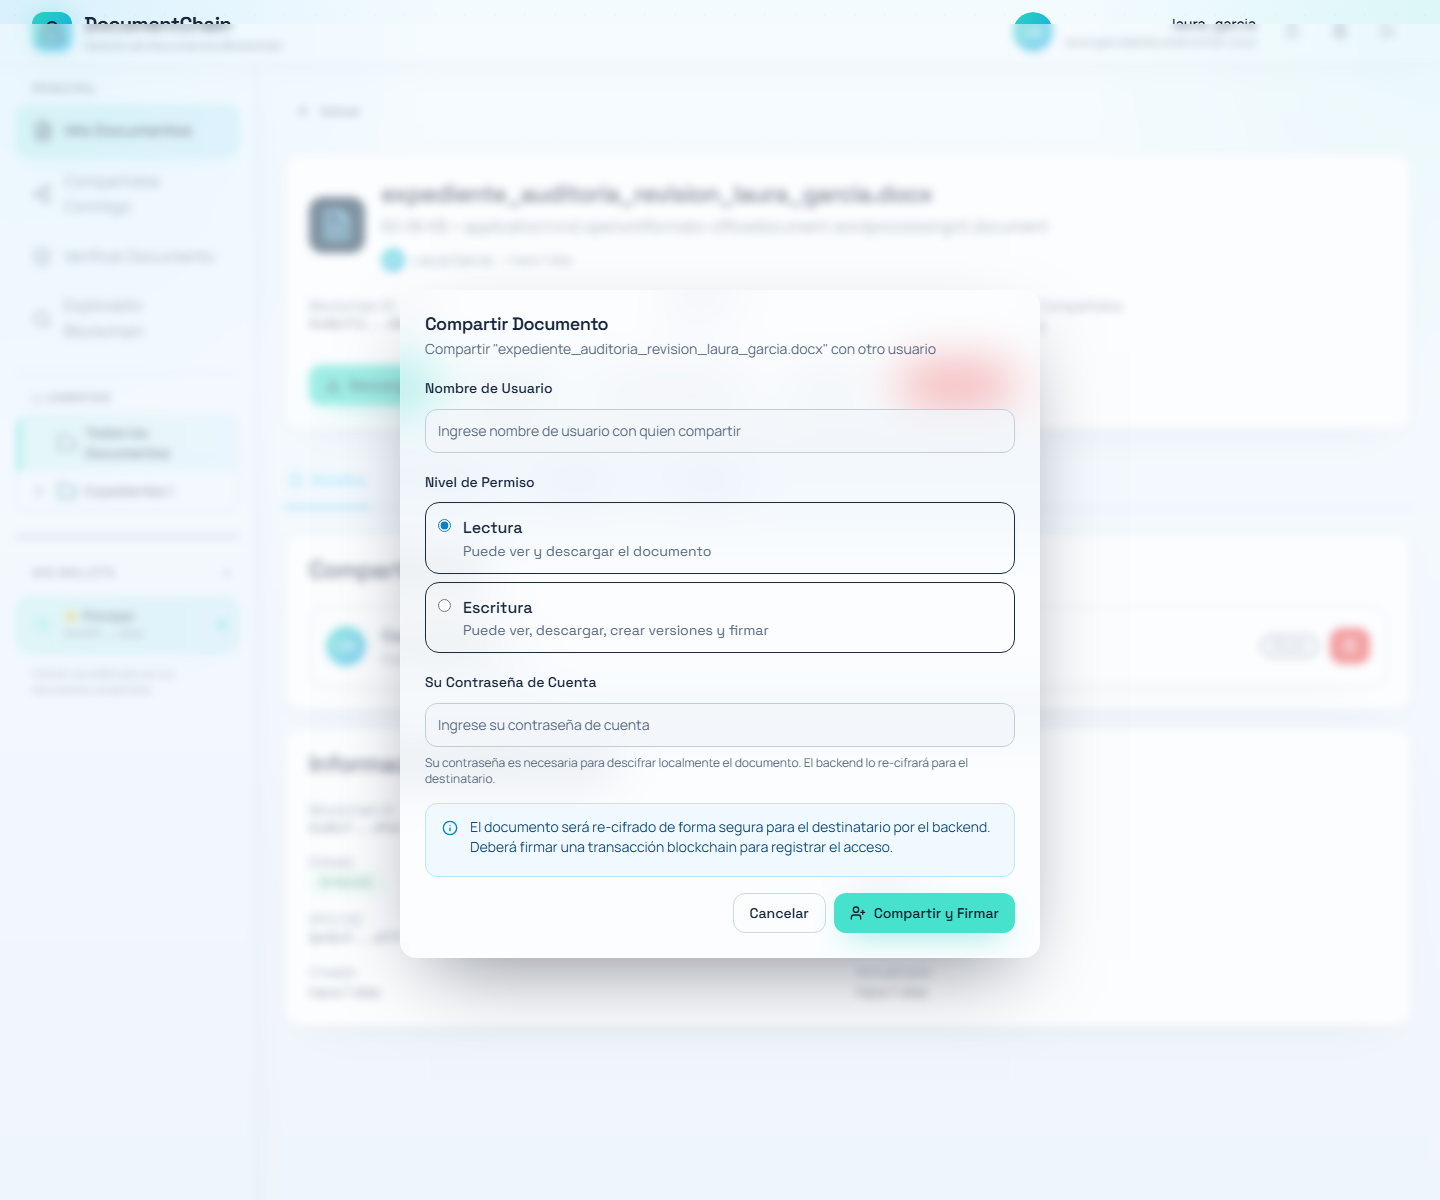
\includegraphics[width=0.8\textwidth]{capturas-ui/share-modal.png}
    \caption{Modal de compartici\'{o}n}
    \label{fig:share}
\end{figure}

\textbf{Resultado esperado}: el destinatario recibe una notificaci\'{o}n y el documento aparece en su secci\'{o}n \textbf{Compartidos Conmigo}. El permiso queda registrado en el contrato inteligente.

\textbf{Posibles errores}:
\begin{itemize}
    \item \textit{``Usuario no encontrado''}: verifique que el correo o wallet introducidos correspondan a una cuenta registrada.
    \item \textit{``Transacci\'{o}n fallida''}: revise que tiene saldo de gas y que la red es la correcta.
\end{itemize}

\subsection{Ver documentos compartidos conmigo}

\textbf{Prop\'{o}sito}: acceder a los documentos que otros usuarios han compartido con su cuenta.

\begin{enumerate}
    \item En la barra lateral izquierda, seleccione \textbf{Compartidos Conmigo}.
    \item Se mostrar\'{a} un listado con los documentos a los que tiene acceso, indicando el propietario original y su rol (Lector o Editor).
    \item Pulse sobre cualquier documento para ver su detalle, historial de versiones o firmas, seg\'{u}n los permisos concedidos.
\end{enumerate}

\begin{figure}[H]
    \centering
    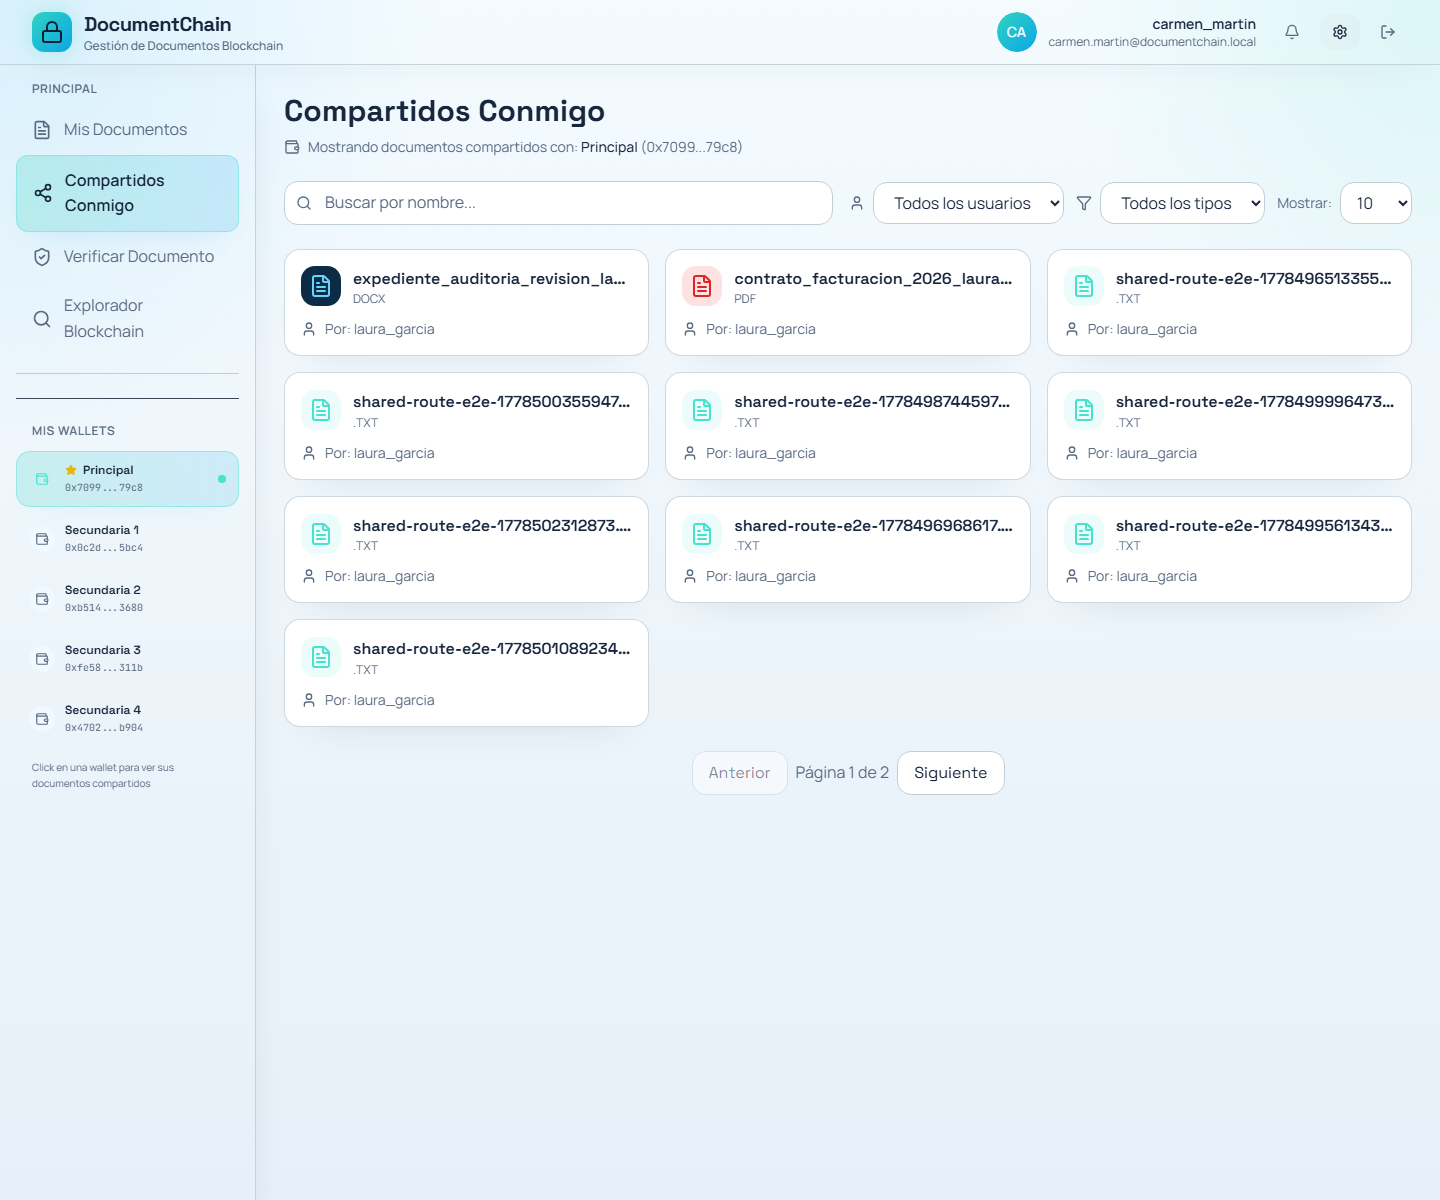
\includegraphics[width=0.9\textwidth]{capturas-ui/shared-page.png}
    \caption{Listado de documentos compartidos con el usuario}
    \label{fig:shared-page-main}
\end{figure}

\subsection{Revocar acceso}

\textbf{Prop\'{o}sito}: retirar los permisos concedidos previamente a un usuario.

\begin{enumerate}
    \item Abra el detalle del documento propio y vaya a la pesta\~{n}a \textbf{Compartir} o \textbf{Permisos}.
    \item Localice al usuario en la lista de destinatarios.
    \item Pulse el icono de papelera o el bot\'{o}n \textbf{Revocar} junto a su nombre.
    \item Confirme la acci\'{o}n y firme la transacci\'{o}n blockchain si se solicita.
\end{enumerate}

\textbf{Resultado esperado}: el usuario perder\'{a} el acceso inmediatamente y el documento desaparecer\'{a} de su lista de compartidos.

% ============================================================
\section{Auditor\'{i}a y verificaci\'{o}n}
% ============================================================

DocumentChain garantiza la trazabilidad de cada documento mediante su registro en blockchain. Este apartado explica c\'{o}mo verificar la autenticidad, consultar transacciones y revisar la l\'{i}nea temporal de un archivo.

\subsection{Verificar autenticidad de un documento}

\textbf{Prop\'{o}sito}: confirmar que un documento no ha sido alterado desde su registro y que su propietario y firmas son v\'{a}lidos.

\begin{enumerate}
    \item Acceda a la p\'{a}gina de verificaci\'{o}n p\'{u}blica mediante el enlace compartible o el c\'{o}digo QR del documento, o bien use la opci\'{o}n \textbf{Verificar Documento} en la barra lateral.
    \item Introduzca el identificador del documento (UUID) o escanee el QR.
    \item El sistema mostrar\'{a}:
    \begin{itemize}
        \item Estado de verificaci\'{o}n (v\'{a}lido / alterado / no encontrado).
        \item Propietario registrado.
        \item Hash del contenido en IPFS.
        \item Lista de firmas asociadas con sus respectivas transacciones blockchain.
    \end{itemize}
\end{enumerate}

\begin{figure}[H]
    \centering
    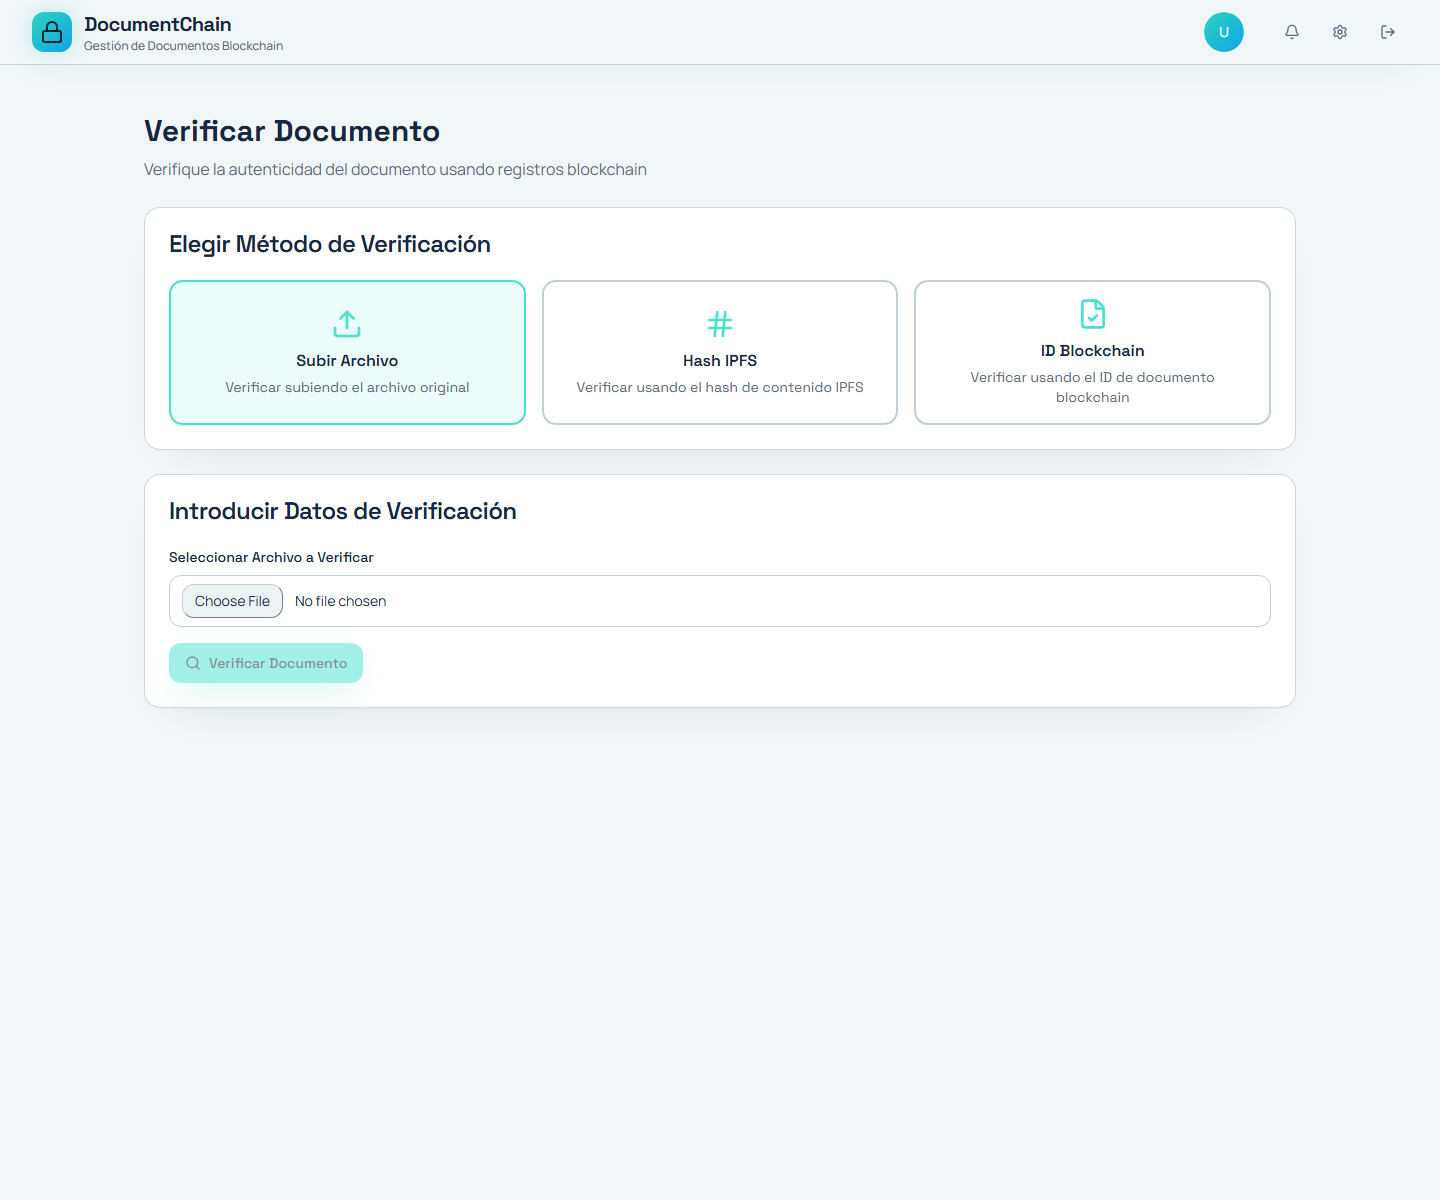
\includegraphics[width=0.8\textwidth]{capturas-ui/verify-page.png}
    \caption{P\'{a}gina de verificaci\'{o}n p\'{u}blica}
    \label{fig:verify}
\end{figure}

\textbf{Resultado esperado}: una confirmaci\'{o}n visual y t\'{e}cnica de la integridad del documento. Si el hash actual no coincide con el registrado, el sistema emitir\'{a} una alerta de alteraci\'{o}n.

\subsection{Auditor\'{i}a blockchain}

\textbf{Prop\'{o}sito}: consultar de forma t\'{e}cnica todas las transacciones y eventos relacionados con un documento.

\begin{enumerate}
    \item Desde el detalle del documento, pulse \textbf{Ver en blockchain} o acceda a \textbf{Explorador Blockchain} desde la barra lateral.
    \item Se mostrar\'{a} una tabla con los eventos registrados en el contrato inteligente:
    \begin{itemize}
        \item Tipo de evento (registro, firma, versi\'{o}n, transferencia, permiso).
        \item Direcci\'{o}n de la wallet que origin\'{o} la transacci\'{o}n.
        \item Hash de la transacci\'{o}n (TxHash).
        \item N\'{u}mero de bloque y marca temporal.
    \end{itemize}
    \item Puede copiar el TxHash para verificarlo en un explorador externo si la red es p\'{u}blica.
\end{enumerate}

\begin{figure}[H]
    \centering
    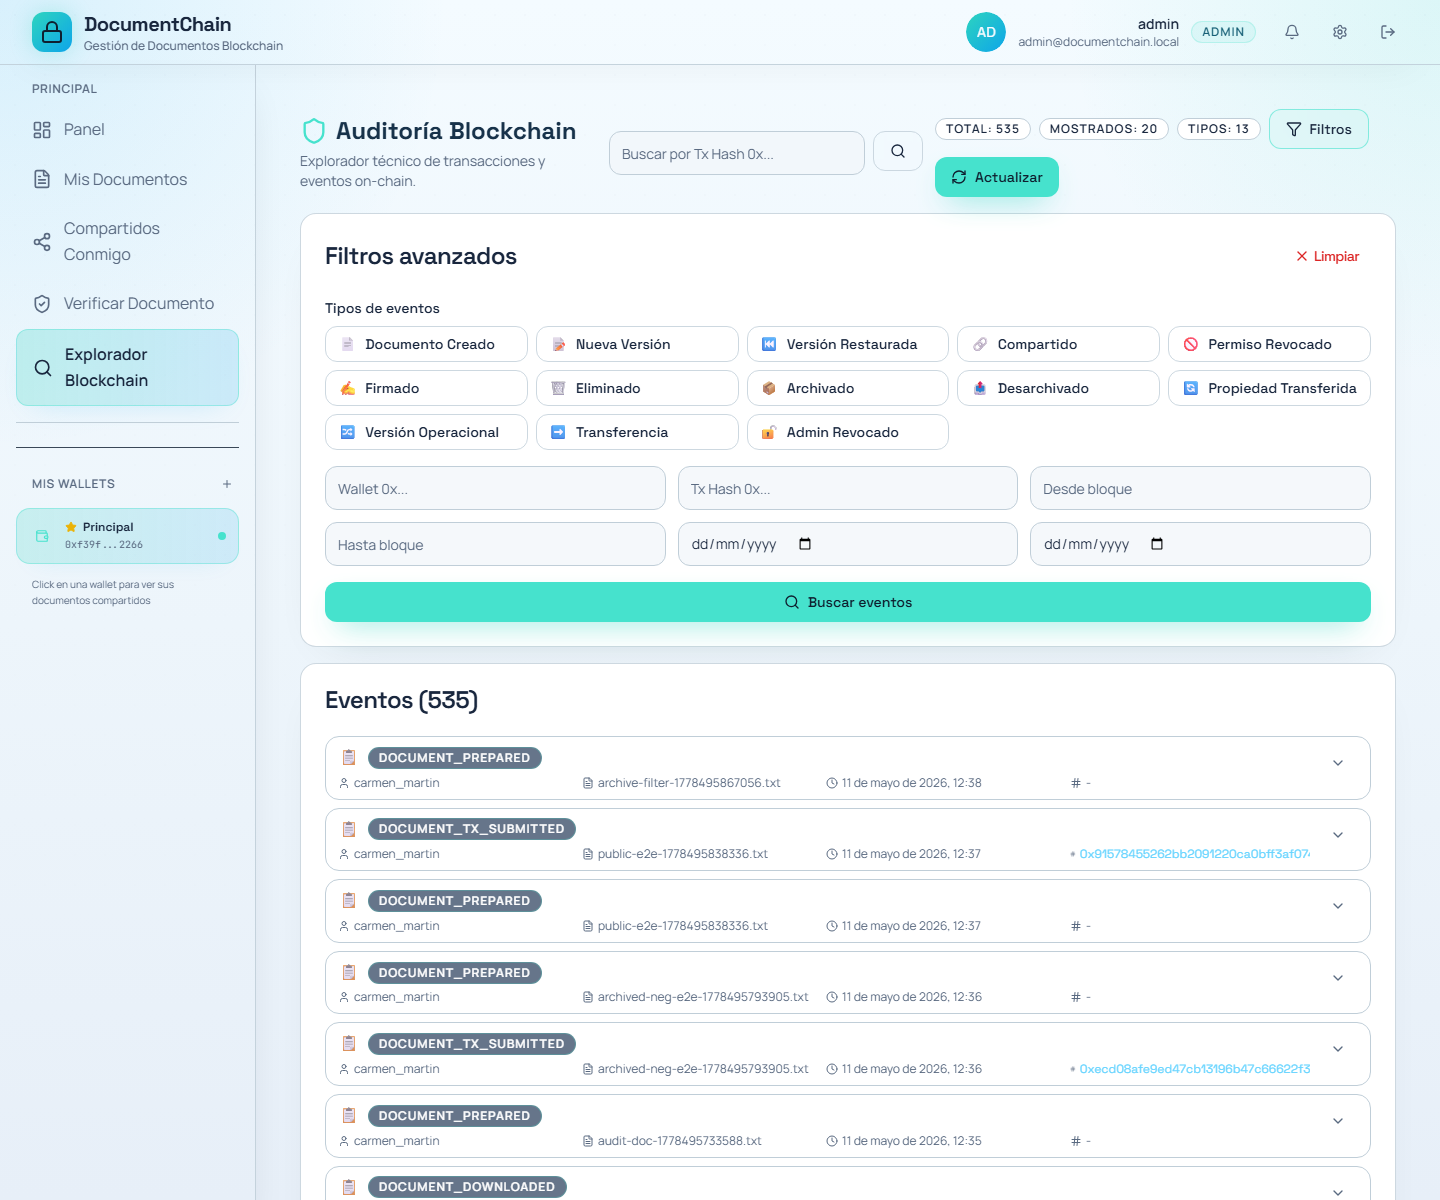
\includegraphics[width=0.9\textwidth]{capturas-ui/blockchain-auditor.png}
    \caption{Vista de auditor\'{i}a blockchain}
    \label{fig:blockchain-auditor-main}
\end{figure}

\subsection{L\'{i}nea temporal (timeline) del documento}

\textbf{Prop\'{o}sito}: visualizar de forma cronol\'{o}gica todas las acciones realizadas sobre un documento.

\begin{enumerate}
    \item Abra el detalle del documento y seleccione la pesta\~{n}a \textbf{Timeline} o \textbf{L\'{i}nea temporal}.
    \item Se presentar\'{a} una secuencia ordenada de eventos:
    \begin{itemize}
        \item Fecha de creaci\'{o}n.
        \item Subidas de nuevas versiones.
        \item Firmas recibidas.
        \item Cambios de propietario.
        \item Modificaciones de permisos.
    \end{itemize}
    \item Cada evento incluye un enlace directo a su transacci\'{o}n blockchain correspondiente.
\end{enumerate}

\begin{figure}[H]
    \centering
    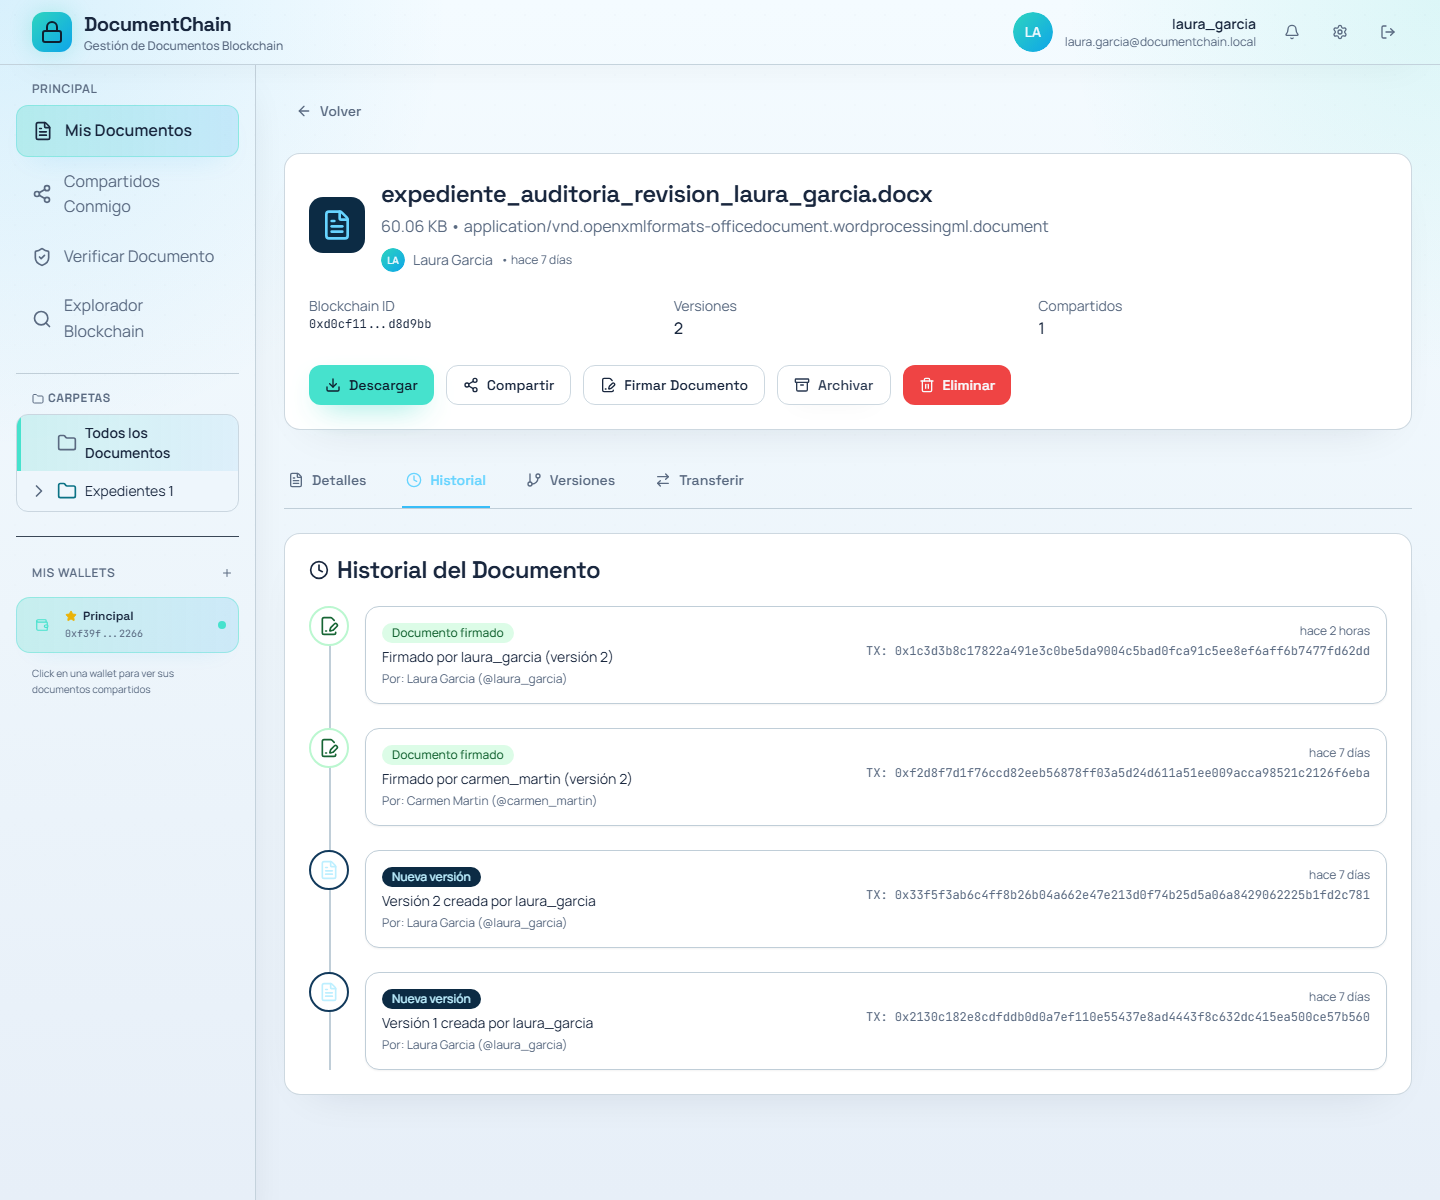
\includegraphics[width=0.9\textwidth]{capturas-ui/timeline-page.png}
    \caption{L\'{i}nea temporal de un documento}
    \label{fig:timeline-main}
\end{figure}

% ============================================================
\section{Gesti\'{o}n de wallets}
% ============================================================

La wallet es la herramienta que permite firmar transacciones blockchain en DocumentChain. Este apartado detalla c\'{o}mo conectar, organizar y gestionar las wallets asociadas a su cuenta.

\subsection{Conectar una wallet}

\textbf{Prop\'{o}sito}: vincular una direcci\'{o}n Ethereum a su cuenta para realizar firmas y registrar operaciones on-chain.

\begin{enumerate}
    \item Acceda a \textbf{Configuraci\'{o}n} $>$ \textbf{Wallets} o pulse el bot\'{o}n \textbf{Conectar wallet} de la cabecera.
    \item Se abrir\'{a} el selector de wallets compatible con EIP-6963.
    \item Elija su proveedor (MetaMask, Rabby, Coinbase Wallet, etc.).
    \item En la extensi\'{o}n de su navegador, confirme la conexi\'{o}n con el sitio web de DocumentChain.
    \item La direcci\'{o}n aparecer\'{a} ahora en la lista de wallets guardadas.
\end{enumerate}

\begin{figure}[H]
    \centering
    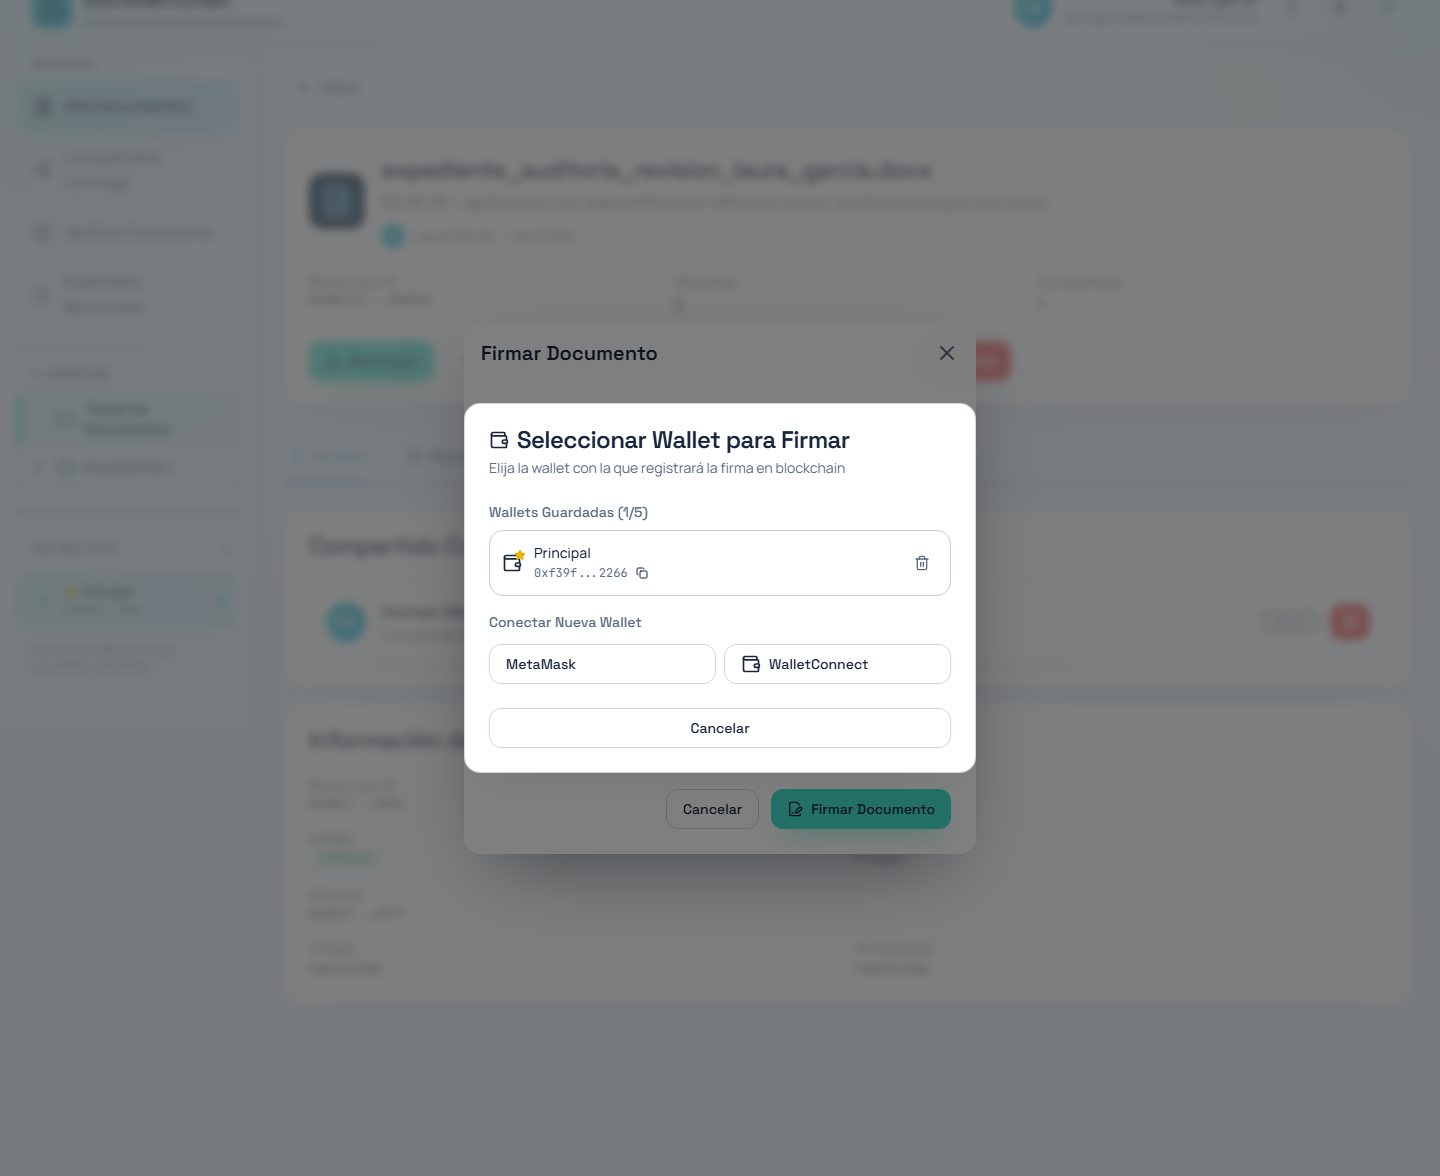
\includegraphics[width=0.8\textwidth]{capturas-ui/wallet-selector-modal.png}
    \caption{Selector de wallets}
    \label{fig:wallet}
\end{figure}

\textbf{Resultado esperado}: la wallet queda vinculada a su cuenta y puede utilizarla para firmar documentos, confirmar comparticiones y registrar transferencias.

\textbf{Posibles errores}:
\begin{itemize}
    \item \textit{``No se detect\'{o} ninguna wallet''}: instale una extensi\'{o}n compatible y recargue la p\'{a}gina.
    \item \textit{``El usuario rechaz\'{o} la conexi\'{o}n''}: desbloquee la wallet y acepte la solicitud de conexi\'{o}n.
\end{itemize}

\subsection{Cambiar wallet principal}

\textbf{Prop\'{o}sito}: establecer qu\'{e} direcci\'{o}n se utiliza por defecto para firmar transacciones.

\begin{enumerate}
    \item Vaya a \textbf{Configuraci\'{o}n} $>$ \textbf{Wallets}.
    \item En la lista de direcciones guardadas, localice la que desea establecer como principal.
    \item Pulse el bot\'{o}n \textbf{Establecer como principal} (icono de estrella).
\end{enumerate}

\textbf{Resultado esperado}: la wallet seleccionada aparecer\'{a} marcada como \textbf{Principal} y se preseleccionar\'{a} autom\'{a}ticamente en los modales de firma.

\subsection{Etiquetar wallet}

\textbf{Prop\'{o}sito}: asignar un nombre descriptivo a cada direcci\'{o}n para identificarlas f\'{a}cilmente.

\begin{enumerate}
    \item En \textbf{Configuraci\'{o}n} $>$ \textbf{Wallets}, pulse el icono de edici\'{o}n junto a la direcci\'{o}n.
    \item Introduzca una etiqueta (por ejemplo, ``Wallet personal'', ``Wallet trabajo'').
    \item Guarde los cambios.
\end{enumerate}

\subsection{Eliminar wallet guardada}

\textbf{Prop\'{o}sito}: desvincular una direcci\'{o}n de su cuenta sin eliminar la wallet del dispositivo.

\begin{enumerate}
    \item En \textbf{Configuraci\'{o}n} $>$ \textbf{Wallets}, pulse el icono de papelera junto a la direcci\'{o}n que desea eliminar.
    \item Confirme la acci\'{o}n.
\end{enumerate}

\textbf{Nota}: eliminar una wallet de DocumentChain no borra la cuenta de la extensi\'{o}n ni los fondos asociados. Simplemente deja de estar vinculada a su perfil en la aplicaci\'{o}n.

% ============================================================
\section{Perfil y configuraci\'{o}n}
% ============================================================

Este apartado agrupa todas las acciones relacionadas con la personalizaci\'{o}n de la cuenta y las preferencias de uso.

\subsection{Acceso al perfil}

\begin{enumerate}
    \item Pulse su avatar o nombre en la cabecera superior.
    \item Seleccione \textbf{Configuraci\'{o}n} o \textbf{Perfil}.
    \item Se abrir\'{a} una p\'{a}gina con pesta\~{n}as organizadas por categor\'{i}as.
\end{enumerate}

\subsection{Cambiar avatar}

\begin{enumerate}
    \item En la pesta\~{n}a \textbf{Perfil}, haga clic sobre su imagen actual.
    \item Seleccione un archivo de imagen desde su dispositivo (formatos JPG, PNG; tama\~{n}o m\'{a}ximo recomendado 2 MB).
    \item El sistema redimensionar\'{a} autom\'{a}ticamente la imagen.
    \item Guarde los cambios.
\end{enumerate}

\subsection{Actualizar datos personales}

\begin{enumerate}
    \item En la pesta\~{n}a \textbf{Perfil}, modifique los campos disponibles: nombre completo, biograf\'{i}a (si aplica), etc.
    \item Si cambia el correo electr\'{o}nico, deber\'{a} verificarlo nuevamente siguiendo el proceso descrito en la secci\'{o}n 2.3.
    \item Pulse \textbf{Guardar cambios}.
\end{enumerate}

\subsection{Cambiar contrase\~{n}a}

\begin{enumerate}
    \item Vaya a \textbf{Configuraci\'{o}n} $>$ \textbf{Seguridad}.
    \item Pulse \textbf{Cambiar contrase\~{n}a}.
    \item Introduzca su contrase\~{n}a actual.
    \item Introduzca la nueva contrase\~{n}a y conf\'{i}rmela.
    \item Pulse \textbf{Actualizar}.
\end{enumerate}

\textbf{Requisito}: la nueva contrase\~{n}a debe cumplir los mismos criterios de fortaleza que en el registro.

\subsection{Preferencias de notificaci\'{o}n}

\textbf{Prop\'{o}sito}: controlar qu\'{e} eventos del sistema generan alertas.

\begin{enumerate}
    \item Acceda a \textbf{Configuraci\'{o}n} $>$ \textbf{Notificaciones}.
    \item Active o desactive las categor\'{i}as disponibles:
    \begin{itemize}
        \item \textbf{Correo electr\'{o}nico}: notificaciones de comparticiones, firmas, cambios de versi\'{o}n.
        \item \textbf{En aplicaci\'{o}n}: alertas en tiempo real dentro de DocumentChain.
        \item \textbf{Blockchain}: avisos cuando una transacci\'{o}n se confirma o falla.
    \end{itemize}
    \item Guarde las preferencias.
\end{enumerate}

\begin{figure}[H]
    \centering
    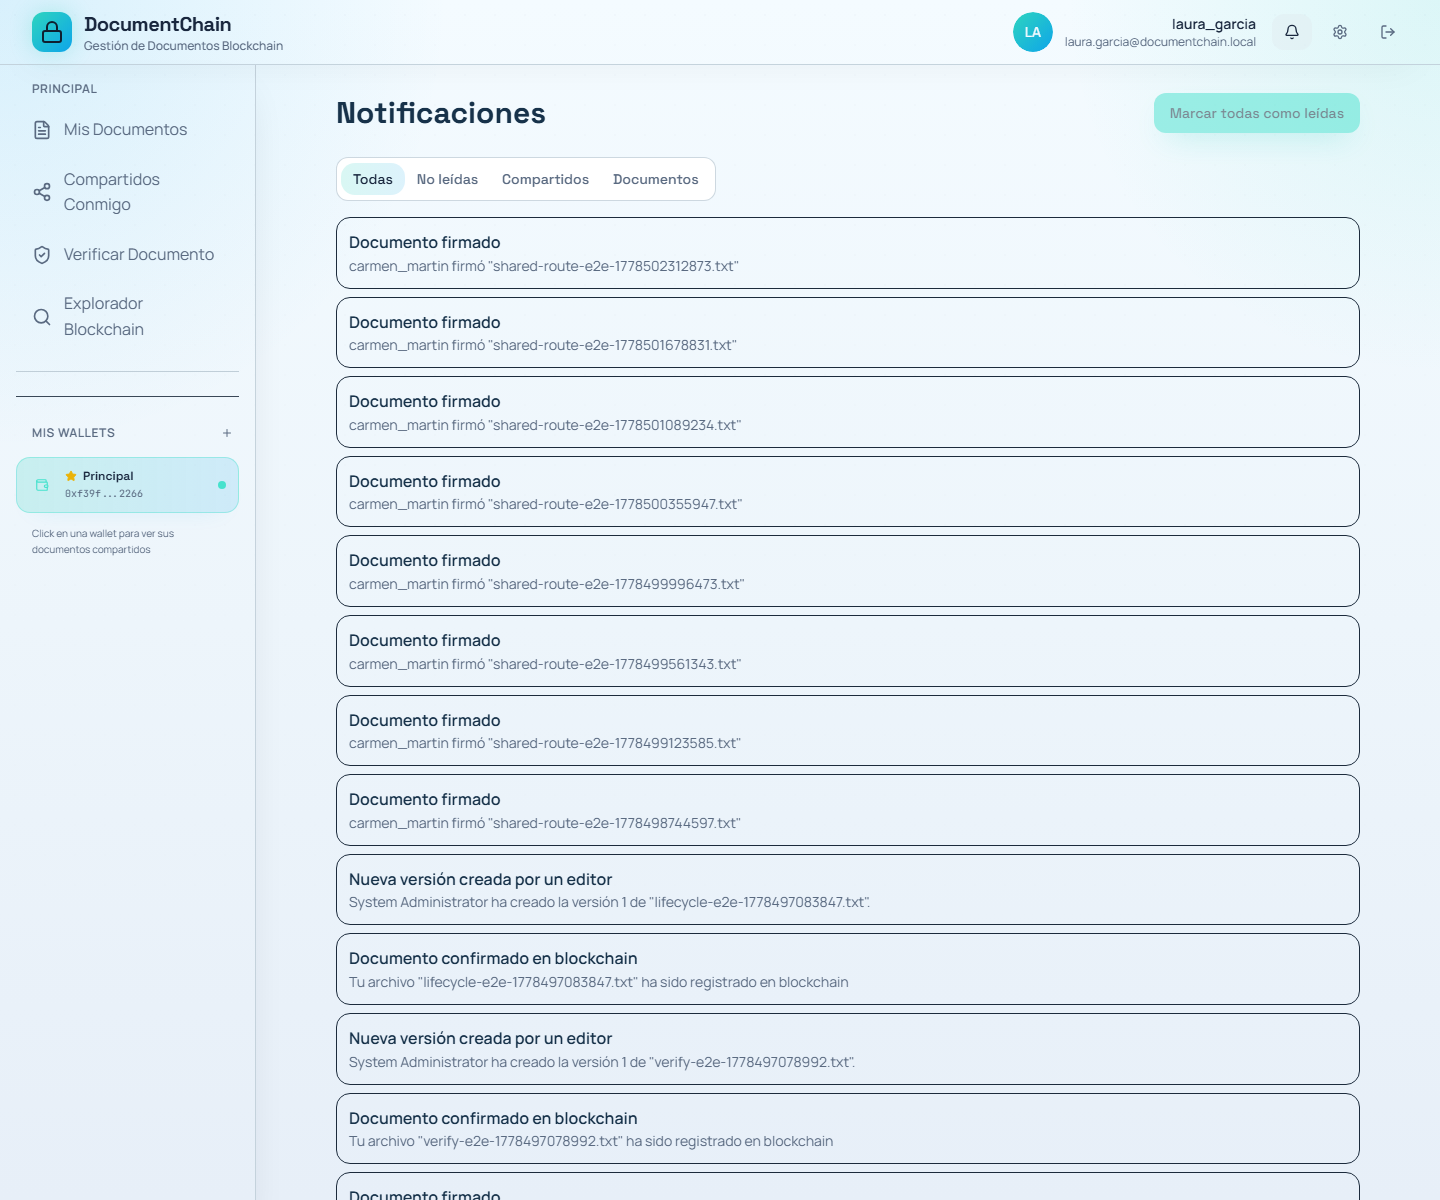
\includegraphics[width=0.75\textwidth]{capturas-ui/notifications-page.png}
    \caption{Centro de notificaciones y preferencias}
    \label{fig:notifications-page}
\end{figure}

\subsection{Gestionar wallets enlazadas}

Consulte el cap\'{i}tulo 8 para el detalle completo de conexi\'{o}n, etiquetado y eliminaci\'{o}n de wallets. Desde el perfil puede acceder r\'{a}pidamente a la misma secci\'{o}n.

\subsection{Seguridad y eliminaci\'{o}n de cuenta}

Para actualizar la contrase\~{n}a o tramitar la eliminaci\'{o}n permanente, siga las instrucciones de la secci\'{o}n 2.5 (Seguridad de cuenta y eliminaci\'{o}n).

% ============================================================
\section{Panel de administraci\'{o}n}
% ============================================================

El panel de administraci\'{o}n est\'{a} reservado a usuarios con rol \texttt{ADMIN}. Permite gestionar el estado global del sistema, supervisar usuarios y consultar logs de auditor\'{i}a.

\subsection{Acceso al panel}

\begin{enumerate}
    \item Inicie sesi\'{o}n con una cuenta que tenga privilegios de administrador.
    \item En la barra lateral, seleccione \textbf{Panel de Administraci\'{o}n} o acceda directamente a \texttt{/app/dashboard}.
\end{enumerate}

\subsection{Estad\'{i}sticas globales}

La pantalla de resumen muestra m\'{e}tricas en tiempo real del sistema:

\begin{itemize}
    \item N\'{u}mero total de usuarios registrados, administradores y usuarios regulares.
    \item N\'{u}mero total de documentos subidos, archivados y eliminados.
    \item Actividad reciente (\'{u}ltimas firmas, subidas y registros blockchain).
    \item Espacio de almacenamiento utilizado en IPFS.
\end{itemize}

\begin{figure}[H]
    \centering
    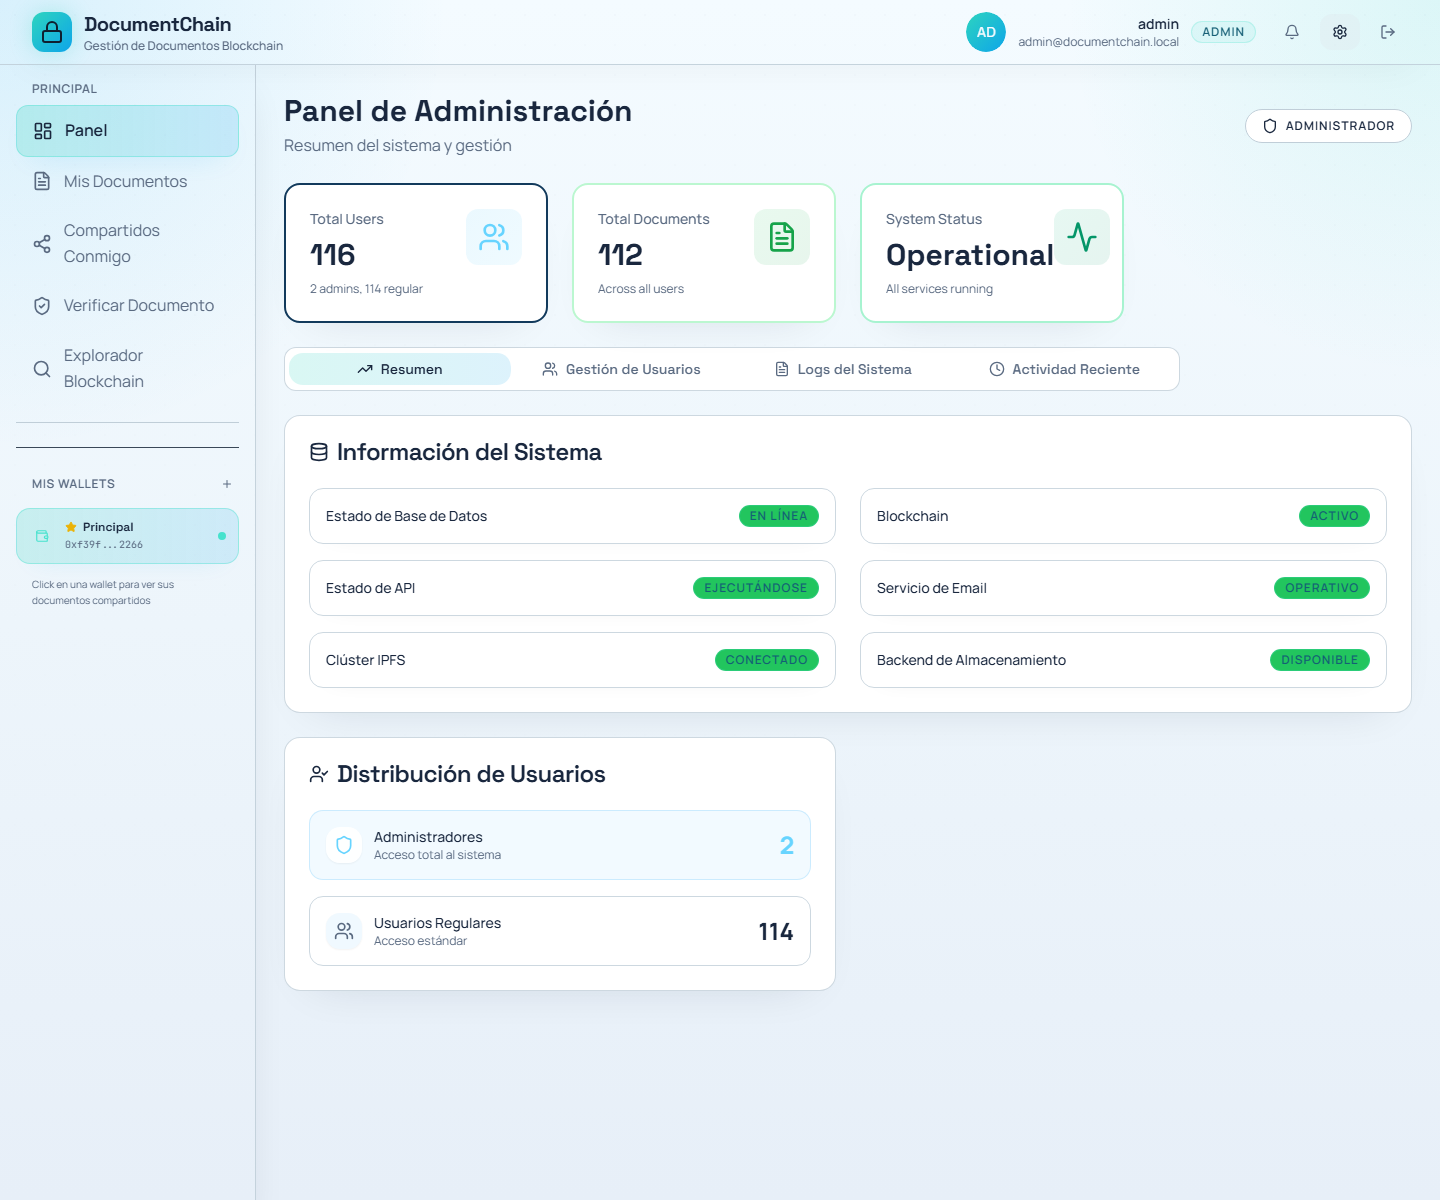
\includegraphics[width=0.8\textwidth]{capturas-ui/admin-dashboard.png}
    \caption{Panel de administraci\'{o}n}
    \label{fig:admin}
\end{figure}

\subsection{Listar y gestionar usuarios}

\begin{enumerate}
    \item En el men\'{u} lateral del panel, seleccione \textbf{Usuarios}.
    \item Se mostrar\'{a} un listado con:
    \begin{itemize}
        \item Nombre de usuario y correo electr\'{o}nico.
        \item Rol actual (Usuario o Administrador).
        \item Fecha de registro, n\'{u}mero de documentos, wallets y sesiones activas.
        \item Datos ampliados al desplegar cada fila del usuario.
    \end{itemize}
    \item Puede aplicar filtros por nombre o rol, y buscar usuarios espec\'{i}ficos.
\end{enumerate}

\begin{figure}[H]
    \centering
    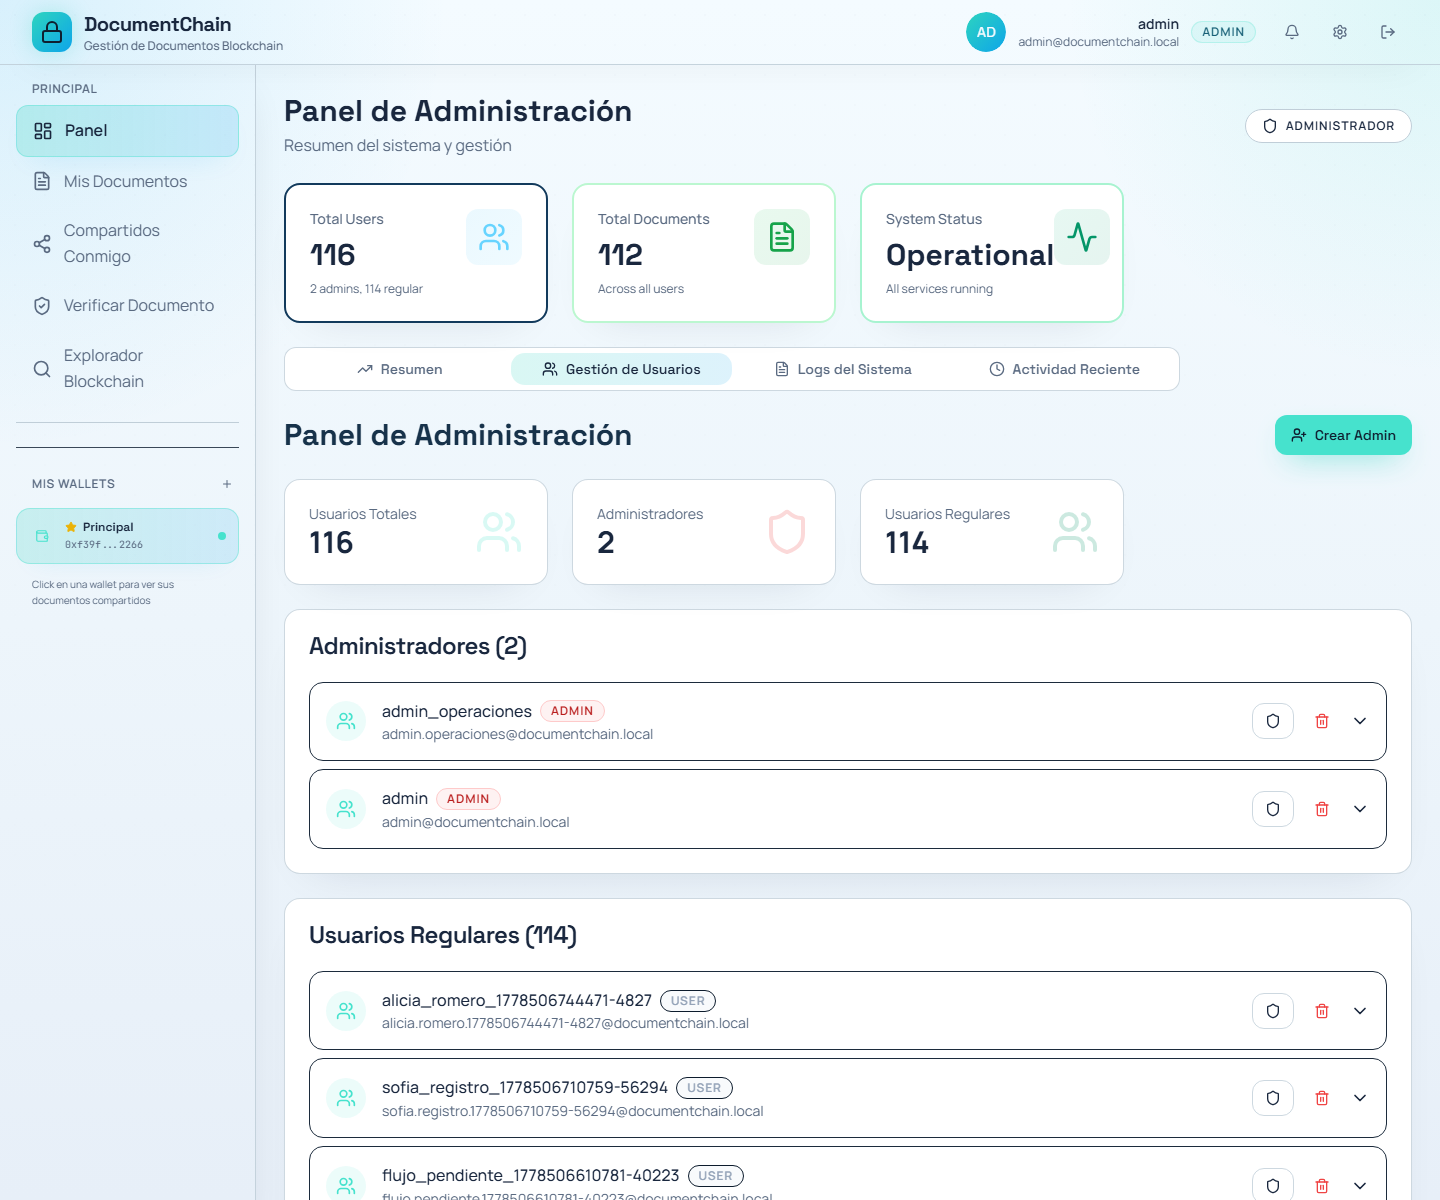
\includegraphics[width=0.9\textwidth]{capturas-ui/admin-users-tab.png}
    \caption{Gesti\'{o}n de usuarios en el panel de administraci\'{o}n}
    \label{fig:admin-users-main}
\end{figure}

\subsection{Gestionar roles}

\textbf{Prop\'{o}sito}: promover un usuario a administrador o revocar dicho privilegio.

\begin{enumerate}
    \item Localice al usuario en el listado.
    \item Pulse \textbf{Editar rol}.
    \item Seleccione \textbf{ADMIN} o \textbf{USER}.
    \item Confirme el cambio.
\end{enumerate}

\textbf{Advertencia}: los administradores tienen acceso al panel de control y a logs sensibles. Asigne este rol con cautela.

\subsection{Eliminar usuarios}

\begin{itemize}
    \item \textbf{Eliminar}: borra la cuenta de forma permanente desde el panel de administraci\'{o}n. La acci\'{o}n requiere confirmaci\'{o}n expl\'{i}cita y debe reservarse para incidencias justificadas.
\end{itemize}

\subsection{Crear cuentas administradoras}

\textbf{Prop\'{o}sito}: incorporar nuevos administradores cuando sea necesario ampliar el equipo de operaci\'{o}n del sistema.

\begin{enumerate}
    \item En el panel de administraci\'{o}n, utilice la acci\'{o}n \textbf{Crear administrador}.
    \item Introduzca los datos de la nueva cuenta.
    \item Revise el rol asignado y confirme la operaci\'{o}n.
    \item El nuevo administrador podr\'{a} acceder al panel tras verificar su correo e iniciar sesi\'{o}n.
\end{enumerate}

\textbf{Resultado}: la nueva cuenta queda registrada con permisos administrativos y pasa a formar parte del panel de gesti\'{o}n.

\subsection{Logs de auditor\'{i}a}

\textbf{Prop\'{o}sito}: revisar todas las operaciones realizadas en el sistema para fines de supervisi\'{o}n y seguridad.

\begin{enumerate}
    \item Acceda a \textbf{Logs} en el panel de administraci\'{o}n.
    \item Filtre por tipo de evento (login, documento, firma, wallet, error), fecha o usuario.
    \item Cada entrada muestra: timestamp, usuario, direcci\'{o}n IP (si aplica), acci\'{o}n realizada y resultado.
\end{enumerate}

\begin{figure}[H]
    \centering
    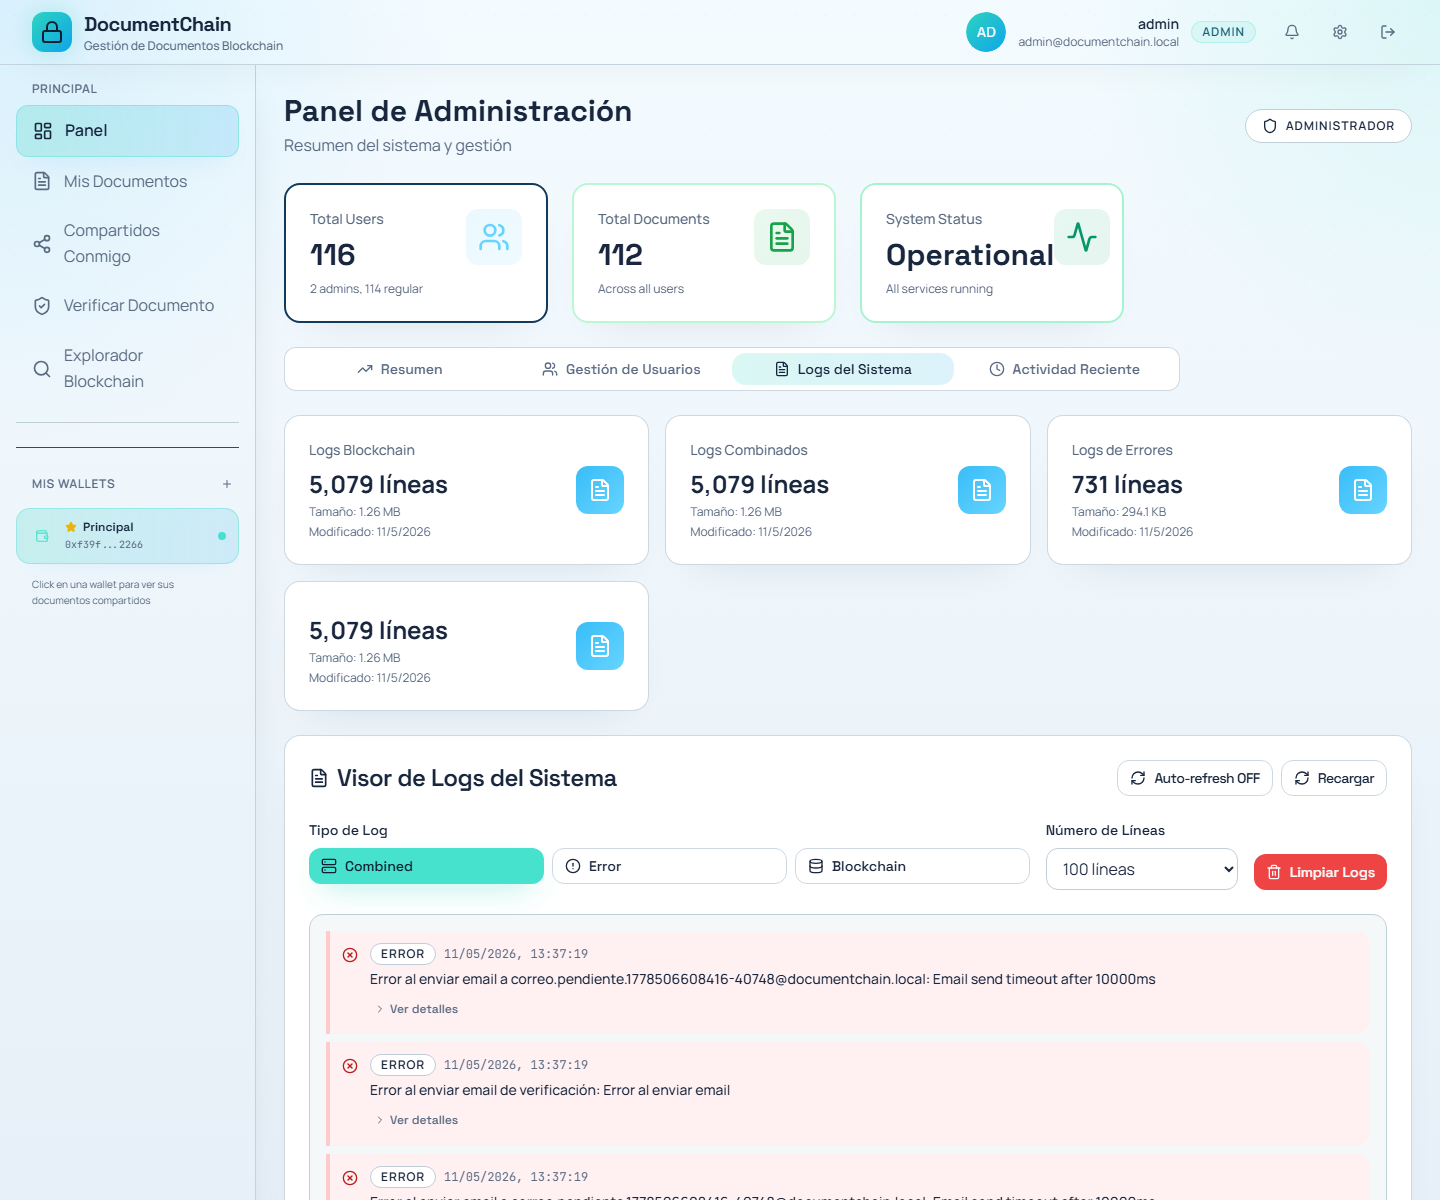
\includegraphics[width=0.9\textwidth]{capturas-ui/admin-logs-tab.png}
    \caption{Visor de logs del sistema}
    \label{fig:admin-logs-main}
\end{figure}

\subsection{Sincronizar administradores con blockchain}

\textbf{Prop\'{o}sito}: asegurar que la lista de administradores del contrato inteligente coincida con la base de datos local.

\begin{enumerate}
    \item En \textbf{Configuraci\'{o}n Avanzada} del panel, pulse \textbf{Sincronizar admins}.
    \item El sistema comparar\'{a} los roles locales con la lista on-chain.
    \item Si detecta diferencias, generar\'{a} las transacciones necesarias para a\~{n}adir o eliminar administradores en el contrato.
    \item Revise y firme cada transacci\'{o}n desde su wallet.
\end{enumerate}

% ============================================================
\section{Adaptaci\'{o}n a dispositivos m\'{o}viles}
% ============================================================

DocumentChain est\'{a} dise\~{n}ado con un enfoque \textit{responsive} que permite su uso desde smartphones y tabletas sin p\'{e}rdida de funcionalidad.

\subsection{Dise\~{n}o responsive}

La interfaz se adapta autom\'{a}ticamente al tama\~{n}o de la pantalla mediante puntos de ruptura (breakpoints) que reorganizan los elementos:

\begin{itemize}
    \item En pantallas grandes (escritorio), se muestra la barra lateral expandida, tablas completas y modales centrados.
    \item En pantallas medianas (tablet), la barra lateral se contrae a iconos y las tablas permiten desplazamiento horizontal.
    \item En pantallas peque\~{n}as (m\'{o}vil), la disposici\'{o}n pasa a una \'{u}nica columna.
\end{itemize}

\subsection{Diferencias en la interfaz m\'{o}vil}

\begin{enumerate}
    \item \textbf{Navegaci\'{o}n}: la barra lateral izquierda se oculta y se accede a ella mediante el bot\'{o}n de men\'{u} hamburguesa situado en la esquina superior derecha.
    \item \textbf{Modales}: las ventanas emergentes ocupan toda la pantalla para facilitar la interacci\'{o}n t\'{a}ctil.
    \item \textbf{Pesta\~{n}as}: cuando el ancho es insuficiente, las pesta\~{n}as permiten desplazamiento horizontal.
    \item \textbf{Acciones}: los botones principales se ubican en la parte inferior de la pantalla para un acceso c\'{o}modo con el pulgar.
    \item \textbf{Wallet m\'{o}vil}: puede conectar su wallet mediante WalletConnect escaneando un c\'{o}digo QR desde la app de MetaMask u otra wallet compatible en su tel\'{e}fono.
\end{enumerate}

\subsection{Recomendaciones de uso en m\'{o}vil}

\begin{itemize}
    \item Utilice la aplicaci\'{o}n en modo vertical para listados y en modo horizontal para revisar documentos con muchas columnas.
    \item Si va a firmar documentos, aseg\'{u}rese de tener instalada la app de su wallet y de que est\'{a} configurada con la red correcta.
    \item Evite borrar los datos de navegaci\'{o}n del navegador m\'{o}vil si tiene documentos privados, por lo que podr\'{i}a perder la clave de descifrado local.
    \item Para descargas grandes, se recomienda usar una conexi\'{o}n Wi-Fi estable.
\end{itemize}

\begin{figure}[H]
    \centering
    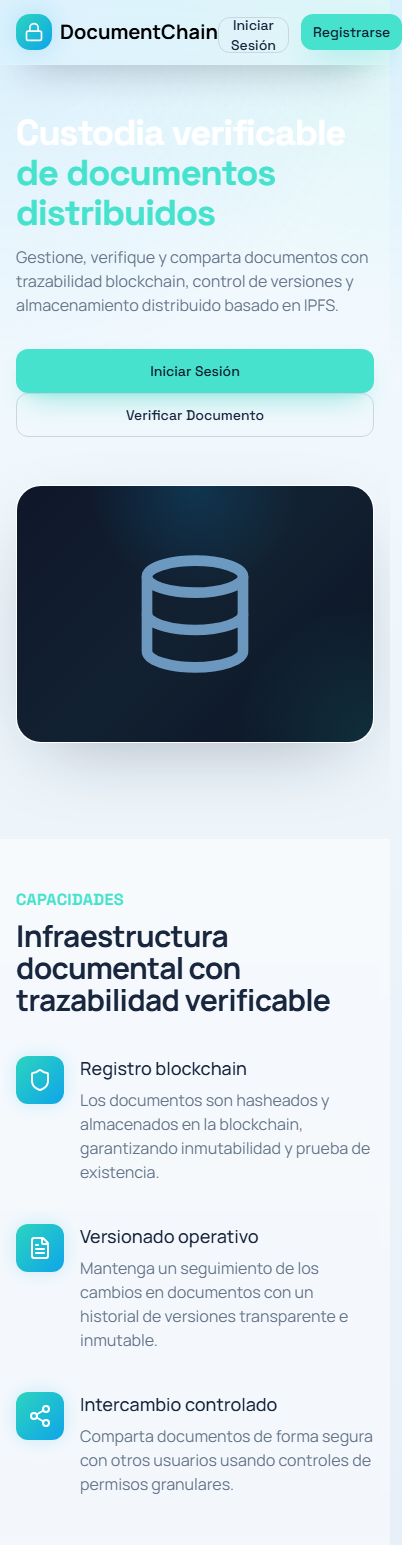
\includegraphics[width=0.45\textwidth]{capturas-ui/mobile-landing.png}
    \caption{Portada p\'{u}blica en dispositivo m\'{o}vil}
    \label{fig:mobile-landing-main}
\end{figure}

\begin{figure}[H]
    \centering
    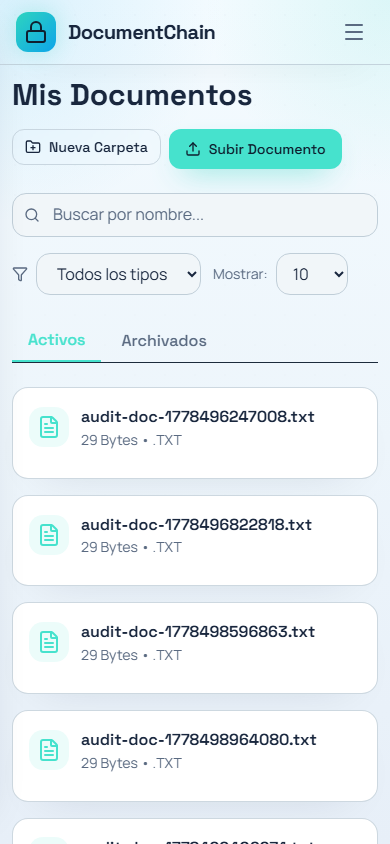
\includegraphics[width=0.45\textwidth]{capturas-ui/mobile-documents-list.png}
    \caption{Listado de documentos en dispositivo m\'{o}vil}
    \label{fig:mobile-documents-main}
\end{figure}

\begin{figure}[H]
    \centering
    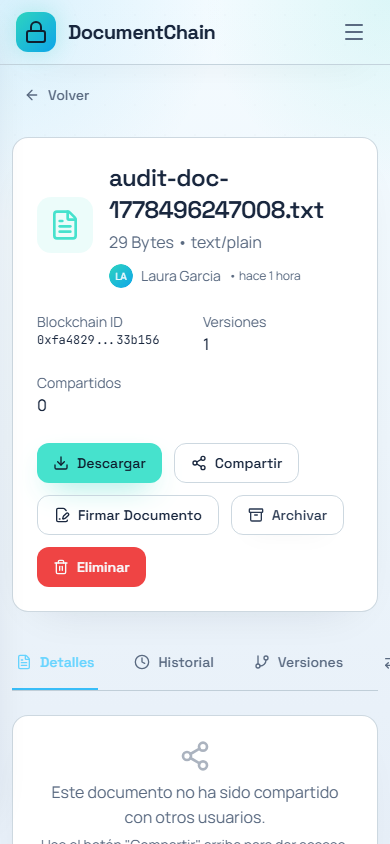
\includegraphics[width=0.45\textwidth]{capturas-ui/mobile-document-detail.png}
    \caption{Detalle de documento en dispositivo m\'{o}vil}
    \label{fig:mobile-document-detail-main}
\end{figure}

\begin{figure}[H]
    \centering
    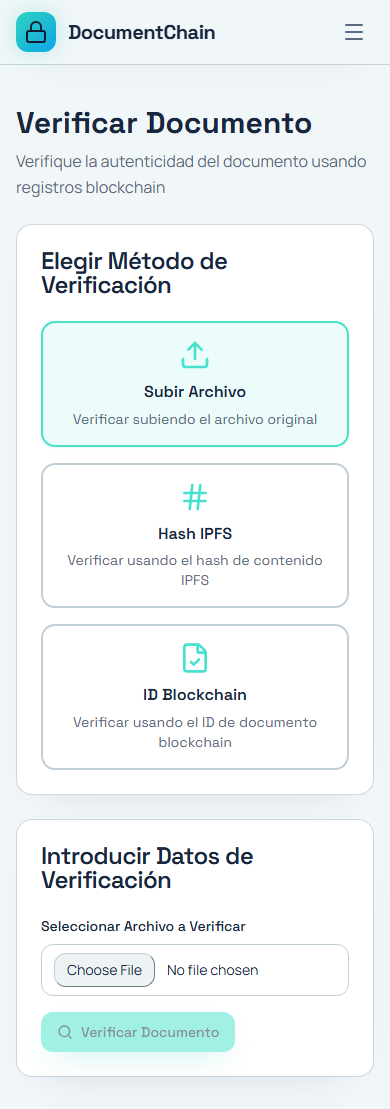
\includegraphics[width=0.45\textwidth]{capturas-ui/mobile-verify.png}
    \caption{Verificaci\'{o}n p\'{u}blica en dispositivo m\'{o}vil}
    \label{fig:mobile-verify-main}
\end{figure}

\begin{figure}[H]
    \centering
    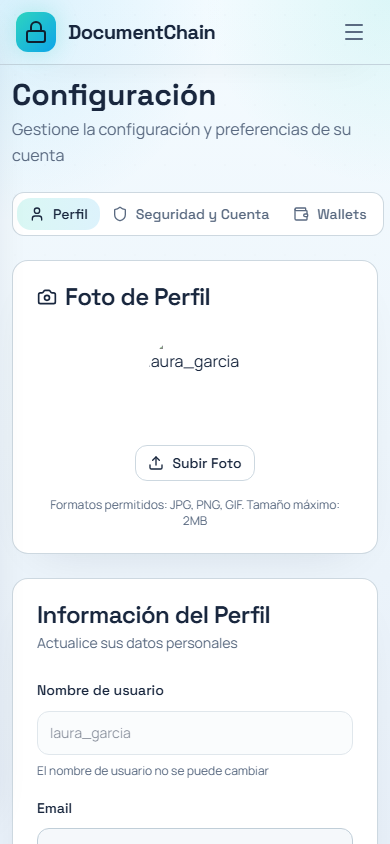
\includegraphics[width=0.45\textwidth]{capturas-ui/mobile-settings.png}
    \caption{Configuraci\'{o}n de cuenta en dispositivo m\'{o}vil}
    \label{fig:mobile-settings-main}
\end{figure}

\begin{figure}[H]
    \centering
    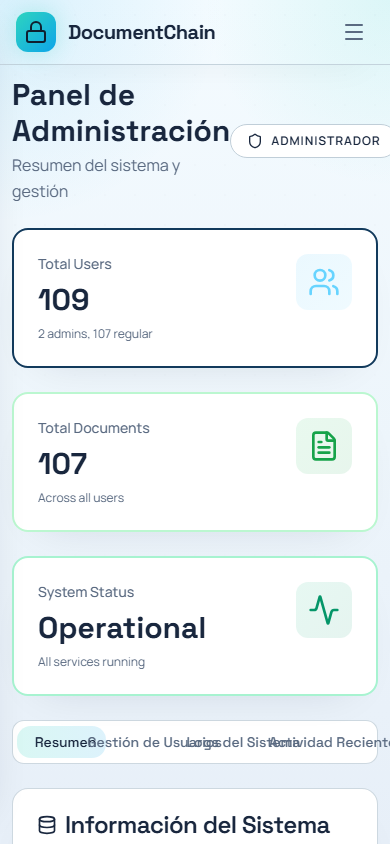
\includegraphics[width=0.45\textwidth]{capturas-ui/mobile-admin-dashboard.png}
    \caption{Panel de administraci\'{o}n en dispositivo m\'{o}vil}
    \label{fig:mobile-admin-main}
\end{figure}

\end{document}
